

%%%%%%%%%%%%%%%%%%%%%%%%%%%%%%%%%%%%%%%%%%%%%%%%%%%%%%%%%%%%%%%%%%%%%%%%%%%%%%%%
% Thesis / Project Report
% LaTeX Template
% Version 2.0 (08/04/16)
%
% Author:
% Parth Ganeriwala
% https://github.com/ParthGaneriwala/BITS-Thesis-Template-Latex
%
% This template is heavily based on the work of Siddhant Shrivastava, Darshit Shah, Steven Gunn and Sunil Patel
% Siddhant Shrivastava
% https://github.com/sidcode/bits-pilani-thesis-template-latex
% Darshit Shah
% https://github.com/darnir/BPHC-LaTeX-Report-Class
% Steven Gunn
% http://users.ecs.soton.ac.uk/srg/softwaretools/document/templates/
% and
% Sunil Patel
% http://www.sunilpatel.co.uk/thesis-template/
%
% License:
% CC BY-NC-SA 4.0 (http://creativecommons.org/licenses/by-nc-sa/4.0/)
%
% Note:
% Make sure to edit document variables in the Thesis.cls file
%
%%%%%%%%%%%%%%%%%%%%%%%%%%%%%%%%%%%%%%%%%%%%%%%%%%%%%%%%%%%%%%%%%%%%%%%%%%%%%%%%

%-------------------------------------------------------------------------------
%	PACKAGES AND OTHER DOCUMENT CONFIGURATIONS
%-------------------------------------------------------------------------------

\documentclass[11pt, a4paper, oneside, british]{Thesis}
% \includeonly{Appendices/Appendix-A} % Paper size, default font size
                                               % and one-sided paper

\graphicspath{{Figures}} % Specifies the directory where pictures are stored

\usepackage[sorting=none,bibstyle=numeric-comp,citestyle=numeric,backend=bibtex,defernumbers=true]{biblatex}  
\addbibresource{References.bib} % Specifies the bibliography file to be used 
\usepackage{physics}  
\usepackage{float} 
\usepackage{bookmark}  
\usepackage{multirow}  
\usepackage{booktabs, makecell}  
\usepackage[table, svgnames]{xcolor}  
\usepackage{siunitx}  
\usepackage{colortbl}  
\usepackage{wrapfig}  
\usepackage{bbm}  
\usepackage{ragged2e}  
\usepackage{array}  
\usepackage{scalerel}  
\usepackage{hyperref}  
\usepackage{mdframed}
\usepackage{tcolorbox}
\usepackage{bbold}
\usepackage{mhchem}
\usepackage{booktabs}
\definecolor{Gray}{gray}{0.9}  
\newlength\mysep   
\setlength\mysep{1cm}  
\DeclareFloatSeparators{mysep}{\hskip\mysep}  

\AtBeginDocument{\RenewCommandCopy\qty\SI}  
\ExplSyntaxOn  
\msg_redirect_name:nnn { siunitx } { physics-pkg } { none }  
\ExplSyntaxOff  

\title{\ttitle}
\makeatletter  
\pdfstringdefDisableCommands{\let\HyPsd@CatcodeWarning\@gobble}  
\makeatother  

\usepackage[T1]{fontenc}
\begin{document}

\frontmatter % Use roman numbering style (i, ii...) for the pre-content pages

\setstretch{1.3} % Line spacing of 1.3

% Define page headers using FancyHdr package and set up for one-sided printing
\fancyhead{} % Clears all page headers and footers
\rhead{\thepage} % Sets the right side header to show the page number
\lhead{} % Clears the left side page header

\pagestyle{fancy} % Finally, use the "fancy" page style to implement the
                  %FancyHdr headers

% Input all the variables used in the document. Please fill out the
% variables.tex file with all your details.
%-------------------------------------------------------------------------------
%	DOCUMENT VARIABLES
%
%	Fill in the lines below to set the various variables for the document
%-------------------------------------------------------------------------------

%-------------------------------------------------------------------------------
% Your thesis title - this is used in the title and abstract
% Command: \ttitle
\thesistitle{Bachelor Thesis}
%-------------------------------------------------------------------------------
% The document type: Thesis / report, etc.
% Command: \doctype
\documenttype{Undergraduate Thesis}
%-------------------------------------------------------------------------------
% Your supervisor's name - this is used in the title page
% Command: \supname
\supervisor{Henry \textsc{Pinto}}
%-------------------------------------------------------------------------------
% The supervisor's position - Used on Certificate
% Command: \suppos
\supervisorposition{Associate PhD Professor}
%-------------------------------------------------------------------------------
% Supervisor's institute
% Command: \supinst
\supervisorinstitute{Yachay Tech University}
\supervisorinstitutecountry{Urcuqui, Ecuador}
%-------------------------------------------------------------------------------
% Your Co-Supervisor's name
% Command: \cosupname
\cosupervisor{Andres \textsc{Garay}}
%-------------------------------------------------------------------------------
% Co-Supervisor's Position - Used on Certificate
% Command: \cosuppos
\cosupervisorposition{Associate PhD Professor}
%-------------------------------------------------------------------------------
% Co-Supervisor's Institute
% Command: \cosupinst
\cosupervisorinstitute{Centro de Investigacion en Materiales Avanzados}
\cosupervisorinstitutecountry{Monterrey, Mexico}
%-------------------------------------------------------------------------------
% Your Examiner's name. Not currently used anywhere.
% Command: \examname
\examiner{}
%-------------------------------------------------------------------------------
% Name of your degree
% Command: \degreename
\degree{Bachelor of Physics}
%-------------------------------------------------------------------------------
% The BITS Course Code for which this report is written
% COmmand: \ccode
\coursecode{BITS F421T}
%-------------------------------------------------------------------------------
% The name of the Course
% Command: \cname
\coursename{Thesis}
%-------------------------------------------------------------------------------
% Your name. Extend manually in case of multiple authors
% Command: \authornames
\authors{J. Gabriel \textsc{Balarezo}}
%-------------------------------------------------------------------------------
% Your ID Number - used on the Title page and abstract
% Command: \idnum
\IDNumber{0106019219}
%-------------------------------------------------------------------------------
% Your address
% Command: \addressnames
\addresses{}
%-------------------------------------------------------------------------------
% Your subject area
% Command: \subjectname
\subject{}
%-------------------------------------------------------------------------------
% Keywords for this report.
% Command: \keywordnames
\keywords{Ab initio calculations, electronic properties, magnetic properties, XGeTe$_3$ monolayers, VASP, PBE,PBESol, Phonopy, Alloy-Theoretic Automated Toolkit, Hubbard U corrections.}
%-------------------------------------------------------------------------------
% University details
% Command: \univname
\university{\texorpdfstring{\href{https://www.bits-pilani.ac.in/Dubai/index.aspx} % URL
                {Yachay Tech University}} % University name
                {Yachay Tech University}}
%-------------------------------------------------------------------------------
% University details, in Capitals
% Command: \UNIVNAME
\UNIVERSITY{\texorpdfstring{\href{https://www.bits-pilani.ac.in/Dubai/index.aspx} % URL
                {Yachay Tech University}} % name in capitals
                {Yachay Tech University}}
                
\UNIVERSITYCOUNTRY{\texorpdfstring{Urcuqui, Ecuador}}
%-------------------------------------------------------------------------------
% Department Details
% Command: \deptname
%\department{\texorpdfstring{\href{https://www.bits-pilani.ac.in/dubai/computerscience/DetofComputerScience} % Your department's URL
%                {Computer Science}} % Your department's name
%                {Computer Science}}
%-------------------------------------------------------------------------------
% Department details, in Capitals
% Command: \DEPTNAME
%\DEPARTMENT{\texorpdfstring{\href{https://www.bits-pilani.ac.in/dubai/computerscience/DetofComputerScience} % Your department's URL
%                {Computer Science}} % Your department's name in capitals
%                {Computer Science}}
%-------------------------------------------------------------------------------
% Research Group Details
% Command: \groupname
\group{\texorpdfstring{\href{Research Group Web Site URL Here (include http://)}
                {Research Group Name}} % Your research group's name
                {Research Group Name}}
%-------------------------------------------------------------------------------
% Research Group Details, in Capitals
% Command: \GROUPNAME
\GROUP{\texorpdfstring{\href{Research Group Web Site URL Here (include http://)}
                {RESEARCH GROUP NAME (IN BLOCK CAPITALS)}}
                {RESEARCH GROUP NAME (IN BLOCK CAPITALS)}}
%-------------------------------------------------------------------------------
% Faculty details
% Command: \facname
\faculty{\texorpdfstring{\href{Faculty Web Site URL Here (include http://www.yachaytech.edu.ec/en/physicsandnanotech/)}
                {School of Physical Sciences and Nanotechnology}}
                {School of Physical Sciences and Nanotechnology}}
%-------------------------------------------------------------------------------
% Faculty details, in Capitals
% Command: \FACNAME
\FACULTY{\texorpdfstring{\href{Faculty Web Site URL Here (include http://)}
                {FACULTY NAME (IN BLOCK CAPITALS)}}
                {FACULTY NAME (IN BLOCK CAPITALS)}}
%-------------------------------------------------------------------------------


%-------------------------------------------------------------------------------
%   NON-CONTENT PAGES
%-------------------------------------------------------------------------------
\maketitle

\Authorship

\Declaration

\Dedicatory{
To the younger self who dared to dream, \\
and to the present self who refuses to falter.\\
For every sleepless night,\\
 and every quiet triumph along the way.
} 
%\Acknowledgements

\Resumen

\Abstract



% \Quotation{Insert Random Quote here. Publish like a boss.}{Your Name}





%-------------------------------------------------------------------------------
%	LIST OF CONTENTS/FIGURES/TABLES PAGES
%-------------------------------------------------------------------------------

% The page style headers have been "empty" all this time, now use the "fancy"
% headers as defined before to bring them back
\pagestyle{fancy}

\lhead{\emph{Contents}} % Set the left side page header to "Contents"
\tableofcontents % Write out the Table of Contents

% Set the left side page header to "List of Figures"
\lhead{\emph{List of Figures}}
\listoffigures % Write out the List of Figures

 % Set the left side page header to "List of Tables"
\lhead{\emph{List of Tables}}
\listoftables % Write out the List of Tables

%-------------------------------------------------------------------------------
%	ABBREVIATIONS
%-------------------------------------------------------------------------------


%-------------------------------------------------------------------------------
%	PHYSICAL CONSTANTS/OTHER DEFINITIONS
%-------------------------------------------------------------------------------

% \clearpage % Start a new page

% % Set the left side page header to "Physical Constants"
% \lhead{\emph{Physical Constants}}

%  % Include a list of Physical Constants (a four column table)
% \listofconstants{lrcl}
% {
% Speed of Light & $c$ & $=$ & $2.997\ 924\ 58\times10^{8}\ \mbox{ms}^{-\mbox{s}}$ (exact)\\
% % Constant Name & Symbol & = & Constant Value (with units) \\
% }

%-------------------------------------------------------------------------------
%	SYMBOLS
%-------------------------------------------------------------------------------

% \clearpage % Start a new page

% \lhead{\emph{Glossary}} % Set the left side page header to "Symbols"

% \listofnomenclature % List the nomenclature. (We use the glossaries package)

%-------------------------------------------------------------------------------
%	DEDICATION
%-------------------------------------------------------------------------------

\mainmatter % Begin numeric (1,2,3...) page numbering

\pagestyle{fancy} % Return the page headers back to the "fancy" style

% Include the chapters of the thesis as separate files from the Chapters folder
% Uncomment the lines as you write the chapters

% Chapter Template

\chapter{Introduction} % Main chapter title

\label{Chapter1} % Change X to a consecutive number; for referencing this chapter elsewhere, use \ref{ChapterX}

\lhead{Chapter 1. \emph{Introduction}} % Change X to a consecutive number; this is for the header on each page - perhaps a shortened title

%----------------------------------------------------------------------------------------
%	SECTION 1
%----------------------------------------------------------------------------------------

%############################# Introduction #################################
\section{Background}
Concrete is the synthetic material currently produced in volumes larger than any other material on Earth. With an annual consumption of approximately 35 billion metric tonnes, it is only second to water in terms of global usage\supercite{mehta2014concrete, Monteiro2017}. It plays a pivotal role in the construction industry, serving as the backbone for buildings, roads, bridges, dams, and many other infrastructure elements central to modern society. Its widespread adoption is the result of its unique combination of properties, including high compressive strength, durability, versatility, and cost-effectiveness\supercite{mehta2014concrete}, rendering it an important asset that directly influences the quality of life and economic development worldwide\supercite{VanDamme2018, Biernacki2017}. Nevertheless, the massive production and use of concrete come with significant environmental challenges. The production of its main constituent, Portland cement, is responsible for 8-9\% of the global anthropogenic CO$_2$ emissions\supercite{Monteiro2017}. Additionally, around 40\% of produced concrete is employed to repair and maintain existing infrastructure\supercite{mehta2014concrete}, which aggravates the environmental impact of concrete. Therefore, the development of more durable and sustainable concrete is of utmost importance, which requires a better understanding of concrete's composition and microstructure. 

Concrete itself is a composite material and can be regarded as a two-phase system\supercite{mehta2014concrete}---the aggregate phase, composed of particles of varying size and shape; and the binding medium, composed of hydrated cement paste. The latter is, in turn, a heterogeneous mixture of different cement hydration products, with calcium silicate hydrate (C-S-H)\footnote{
Conventional cement chemistry notation: C = CaO, S = SiO$_2$, H = H$_2$O
} being the most abundant and important phase. C-S-H makes up 50 to 60\% of the volume of solids in a hydrated cement paste and is responsible for the majority of the long-term strength and durability of concrete\supercite{mehta2014concrete}. Together, the aggregate and binding phases form a complex microstructure that bridges the nanoscale chemistry of hydration products with the properties of concrete at the engineering scale. Nonetheless, the underlying microstructure-property relationships in concrete are not yet fully understood, hindering our ability to manipulate and tailor its properties for specific applications. 


In this context, numerous efforts have been made to understand and model the properties of C-S-H, owing to its central role in determining the properties of concrete\supercite{Ji2012, Papatzani2015, Qomi2020}. Characterisation techniques---such as X-ray diffraction (XRD)\supercite{Allen2007, Houston2009, Oh2012}, nuclear magnetic resonance (NMR)\supercite{Foley2012, Maddalena2019}, and small angle neutron scattering (SANS)---have provided valuable insights into the structure and composition of C-S-H upon which many molecular models have been developed. The pioneering work of Pellenq \emph{et al.}\supercite{Pellenq2009}---which introduced a realistic molecular model of cement hydrates---paved the way for a wide range of molecular modelling techniques\supercite{AbdolhosseiniQomi2014, Richardson2014, Bauchy2014, Kovacevic2016, KunhiMohamed2018} intended to capture the nanoscale structure and properties of C-S-H accurately. Additionally, the advancement of computational power and the development of efficient molecular dynamics (MD) simulation methods have enabled the exploration of mechanical, thermal, and transport properties of C-S-~H\supercite{
AbdolhosseiniQomi2015, Bahraq2022, Cho2020, Barbhuiya2023} under conditions that are relevant to concrete applications but difficult to replicate experimentally. The upscaling of C-S-H properties can be viewed from a hierarchical multiscale perspective, as illustrated in Figure \ref{fig:figure1}, which highlights the microstructure-property relationships of C-S-H at different scales and the relevance of nanoscale properties to the engineering scale of concrete.
\begin{figure}[H]
    \centering
    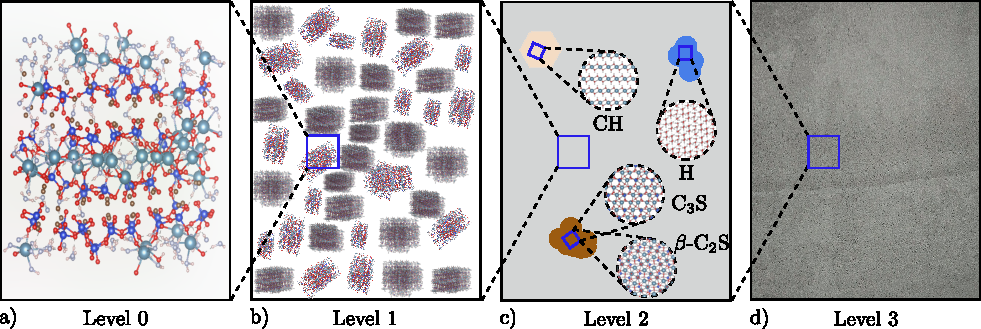
\includegraphics[width=0.9\textwidth]{levels.png}
    \caption{A four-level model representing the upscaling of C-S-H properties from the nanoscale to the engineering scale. (a) snapshot of C-S-H's nanostructure. (b) microstructure of C-S-H created by agglomeration of randomly oriented C-S-H nanoparticles. (c) microtexture of hardened paste composed of hydration products. (d) Macrotexture of cement paste at the engineering scale. Adapted from Ref.\supercite{AbdolhosseiniQomi2015}.}
    \label{fig:figure1}
\end{figure}

Despite the significant progress made in understanding C-S-H at the atomic scale, the inherent complexity of this material makes it challenging to model its structure and properties using classical methods realistically ---primarily molecular dynamics (MD) simulations. Resorting to \emph{ab initio} methods---such as density functional theory (DFT)---can hugely improve the accuracy of these models, but demand high computational resources, making it nearly intractable for real applications\supercite{zotero-item-16}. In this context, machine learning (ML) based concrete research has emerged as a promising approach to address these challenges\supercite{zotero-item-16, Kobayashi2021, Zhu2024}. Trained on large, high-quality \emph{ab initio} datasets, ML models can capture the underlying physics of C-S-H and predict its properties with high accuracy, comparable to that of first-principles methods, while requiring significantly less computational power. 

%-----------------------------------
%	SUBSECTION 1
%-----------------------------------
\section{Problem Statement}
Concrete production is projected to increase by 50\% annually by 2050\supercite{Monteiro2017}, and with no foreseeable alternatives to Portland cement, the urgent need for more sustainable concrete is evident. The development of advanced concrete with enhanced durability and performance could significantly lower the environmental burden. State-of-the-art methods such as machine learning show great potential to accelerate this transition, providing a powerful tool to advance our understanding of concrete's microstructure and properties. 

In this context, this report aims to investigate the performance of a machine learning force field (MLFF) in modelling and predicting the mechanical properties of C-S-H. Such MLFF will be trained and validated
using \emph{ab initio} data, ensuring it captures the complex atomic interactions and structural variability of C-S-H. Ultimately, our goal is to develop a reliable and computationally efficient model that can predict the mechanical properties of C-S-H, thereby supporting concrete research towards a sustainable future.
%-----------------------------------
%	SUBSECTION 2
%-----------------------------------

\section{General and Specific Objectives}
The main goal of this work is to use density functional theory (DFT), \emph{ab initio} molecular dynamics (AIMD), and machine learning (ML) to
develop a machine learning force field (MLFF) for calcium silicate hydrates (C-S-H) to study the mechanical properties of C-S-H. To achieve this, the following specific objectives are defined:
\begin{itemize}
    \item To describe the theoretical foundations of DFT, AIMD, and MLFFs, including key concepts on exchange-correlation functionals such as PBE and PBEsol, and pseudopotentials. 
    \item To perform geometric relaxation on bulk C-S-H model employing the VASP software with the PBEsol functional.
    \item To analyse the electronic structure of C-S-H by computing the density of states (DOS) of C-S-H.
    \item To train, refit, and test an MLFF using AIMD simulations. 
    \item To compute the equation of state (EOS) and mechanical properties of C-S-H using the MLFF and simulated annealing methods.
    \item To evaluate the transferability of the MLFF by computing the thermal expansion coefficient of C-S-H. 
\end{itemize}
%----------------------------------------------------------------------------------------
%	SECTION 2
%----------------------------------------------------------------------------------------

\section{Overview}
The remainder of this report is organised in the following manner: Chapter \ref{Chapter2} introduces the theoretical framework of the computational methods utilised in this work, including DFT, AIMD, and MLFFs. Chapter \ref{Chapter3} presents the methodology employed to generate the results presented in this report, describing the molecular model of C-S-H, the computational setup, and the MLFF generation process. Then, Chapter \ref{Chapter4} presents the results of our computational investigations. Ultimately, Chapter \ref{Chapter5} finalises this report, the main conclusions about the work done are drawn, and the outlook for future work is discussed.

\include{Chapters/Chapter-2-edited}
\chapter{Methodology}
\label{Chapeter3}
\lhead{Chapter 3. \emph{Methodology}}  
This chapter outlines the methodology followed in this work to perform the computational simulations of calcium silicate hydrates (C-S-H). All the calculations were carried out using Density Functional Tight Binding (DFTB+)---primarily in the initial stages---and subsequently with the Vienna Ab-initio Simulation Package (VASP).

We begin by describing the initial C-S-H structure, followed by the 
details of the VASP workflow, emphasising the self-consistent field (SCF) cycle. We then present the main input and output files required for the simulations. Next, we discuss the structure relaxation procedure, which includes an initial relaxation using DFTB+ followed by a full structure relaxation with VASP. Finally, we discuss the generation of the machine learning force field (MLFF), covering the training, refinement, and testing phases. 

\section{Initial CSH Structure}
The structure used for our investigations of calcium silicate hydrates (C-S-H)---from now on referred to as CSH---is the CSH molecular model proposed by Pellenq \emph{et al.}\supercite{Pellenq2009}. We constructed this model with chemical composition as the overriding constraint. As such, the model has a calcium/silicon ratio (C/S) of 1.7, and a density of 2.6 g/cm$^3$; consistent with experimental observations. 

It was derived from a monoclinic periodic cell of dry tobermorite, from which SiO$_2$ groups were removed to achieve an experimental C/S ratio. Thereafter, the structure was relaxed using a core-shell potential model at 0 K. Finally, they carried out a Grand Canonical Monte Carlo simulation of water adsorption at 300 K, reporting a chemical composition of (CaO)$_{1.65}$(SiO$_2$)(H$_2$O)$_{1.75}$. 

The model, shown in Figure \ref{fig:csh_structure}, contains
99 calcium (Ca), 60 silicon (Si), 323 oxygen (O), and 208 hydrogen (H) atoms, making a total of 690 atoms. It is noteworthy that the model is not regarded as a perfect representation of C-S-H, but rather as a good approximation that captures the essential features of cement hydrates.

\begin{figure}[h]
    \centering
    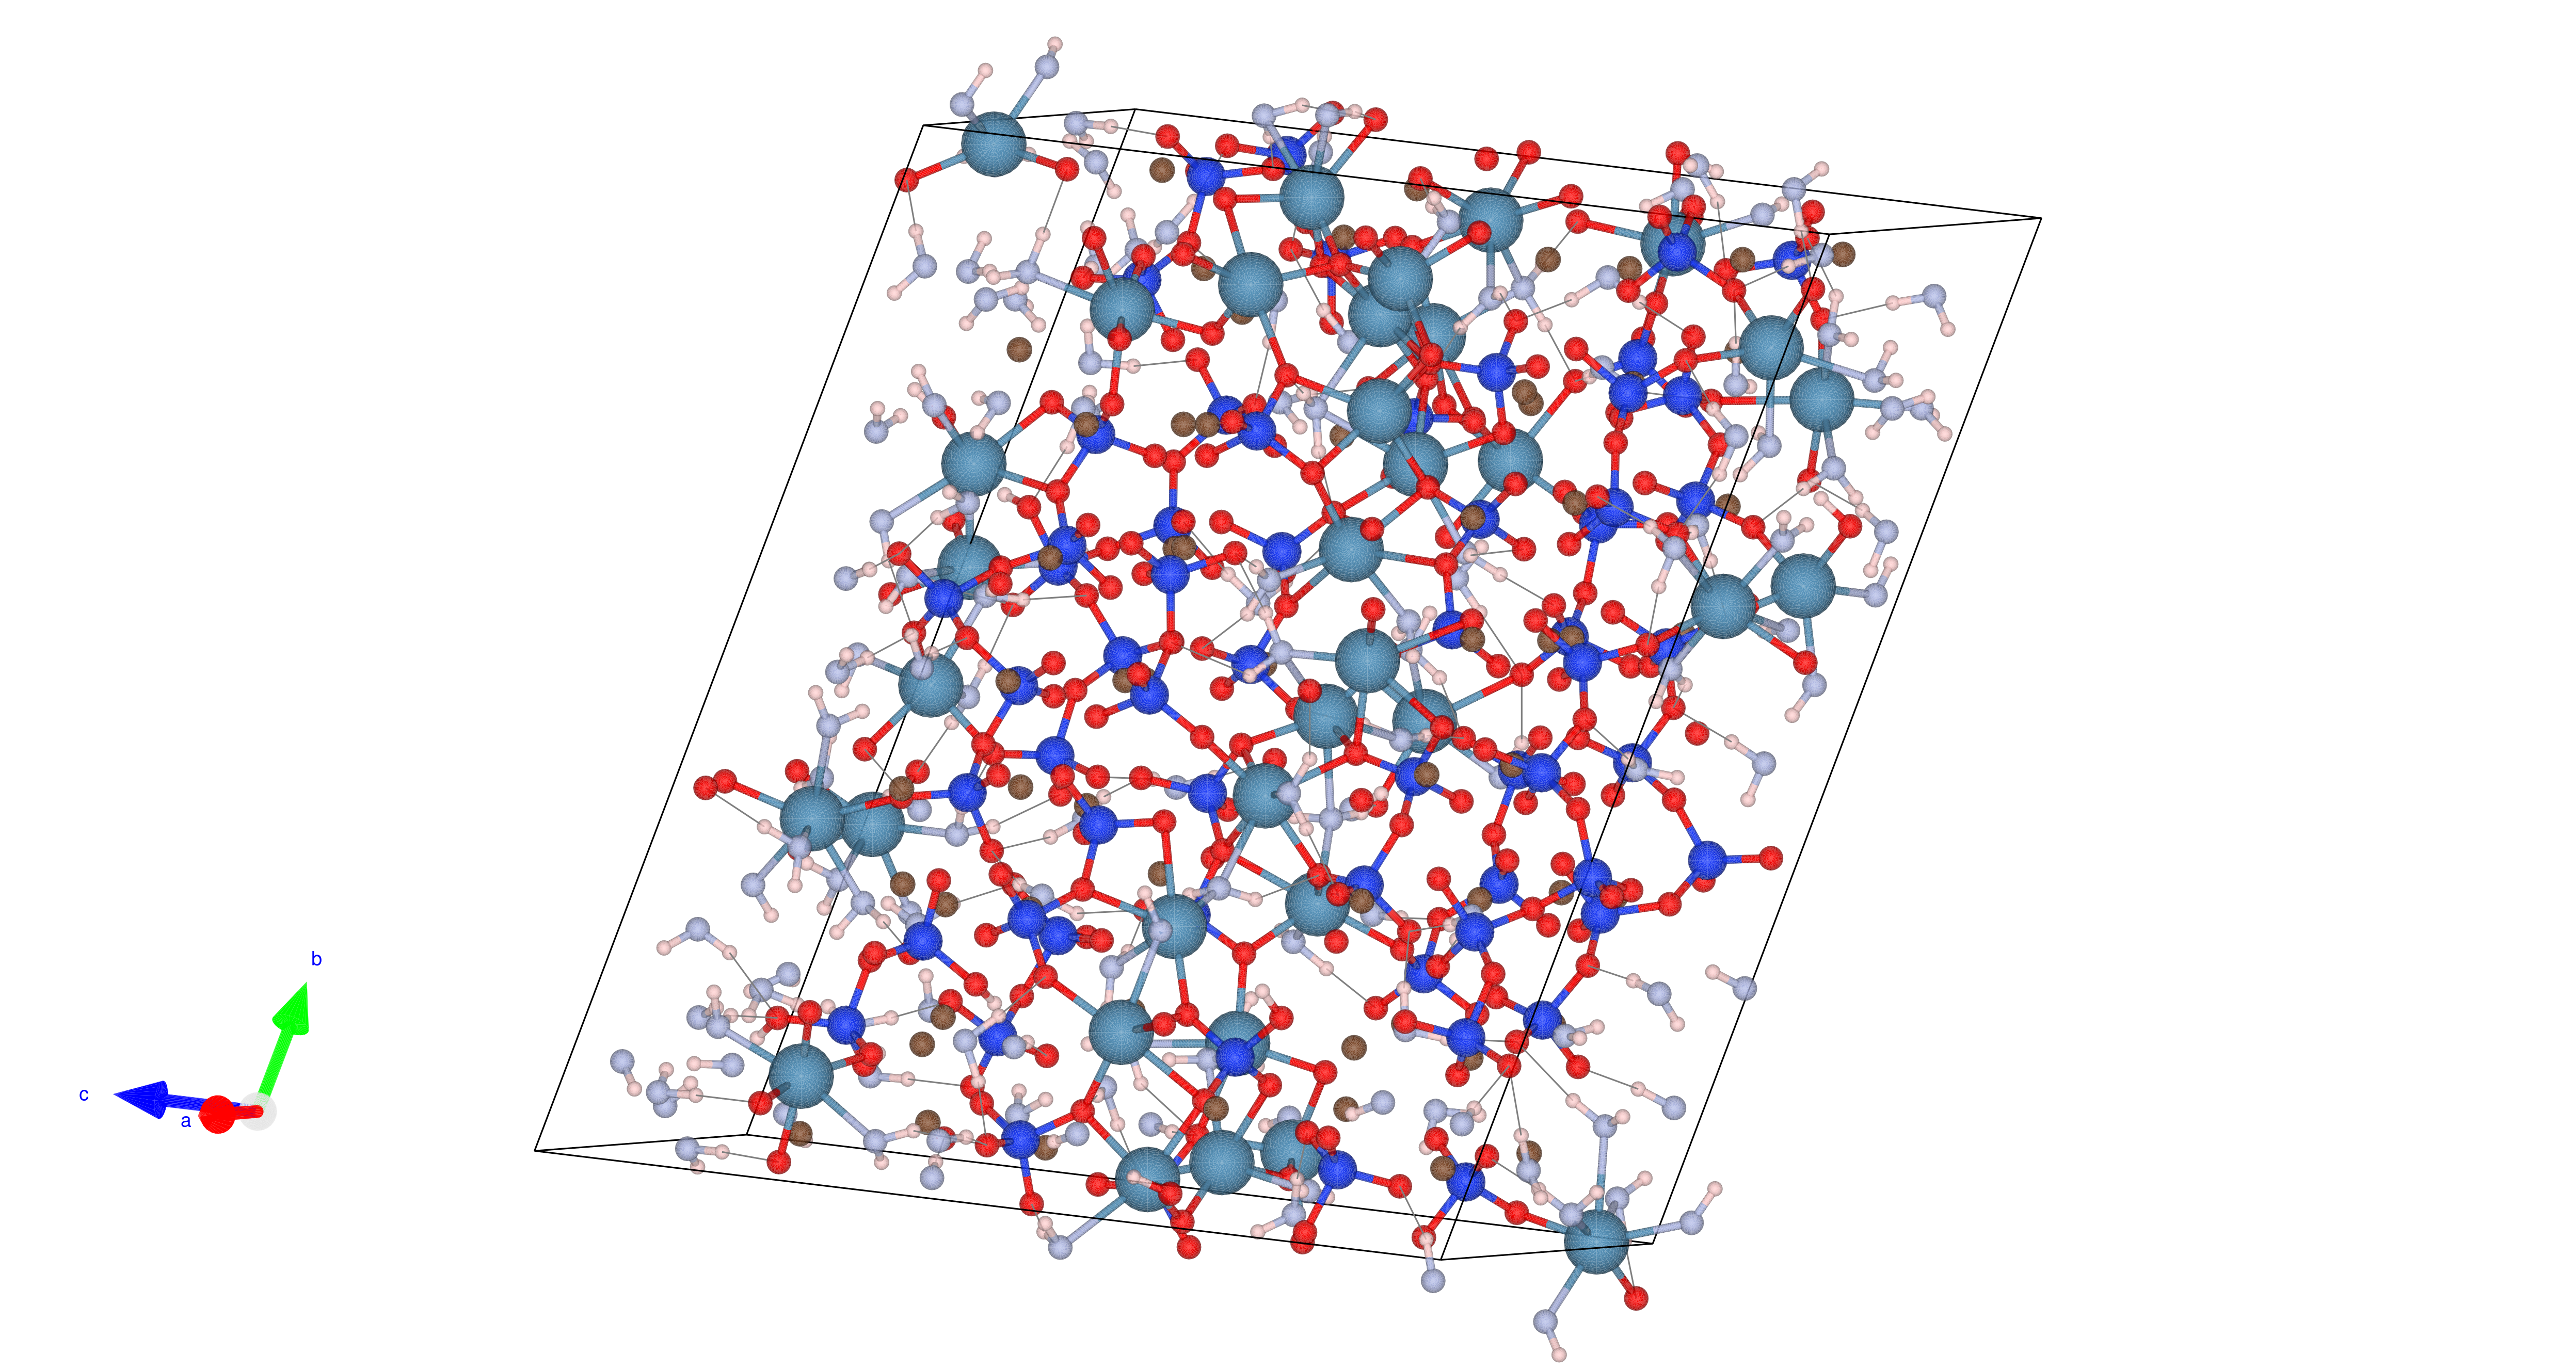
\includegraphics[width=1\textwidth]{POSCAR-extra-colours.png}
    \caption{Molecular model of C-S-H proposed by Ref.\supercite{Pellenq2009}. Lavender and white spheres are oxygen and hydrogen from water molecules, respectively; light blue and brown spheres are inter- and intra-layer calcium ions, respectively; electric blue and red spheres are silicon and oxygen atoms from silica tetrahedra, respectively.}
    \label{fig:csh_structure}
\end{figure}

\section{VASP Workflow}
Most of our calculations were performed using the Vienna Ab Initio Simulation Package (VASP). A central part of the VASP workflow is the self-consistent field (SCF) cycle, illustrated in Figure~\ref{fig:vasp_workflow}. This cycle is essential for structure relaxation, \emph{ab initio} molecular dynamics (AIMD) simulations, and other DFT calculations. We hereby present the main procedure of the SCF cycle:

\begin{itemize}
    \item At the beginning of the cycle, a trial electronic density is generated---either from a previous calculation or from an initial guess. 
    \item The algorithm then proceeds to construct the effective potential, defined as the sum of the Hartree, external, and exchange-correlation potentials. This latter is specified by the user (e.g., PBEsol, HSE06).
    \item VASP then solves the Kohn-Sham equation, generating a new set of single-electron wavefunctions at each iteration. 
    \item A new electronic density is calculated from the wavefunctions. This process repeats until self-consistency is achieved---\emph{i.e.}, the total energy difference between consecutive iterations falls below a predefined tolerance. The user sets this value, and for our calculations, a value of \texttt{EDIFF = 1E-4} was used. 
\end{itemize}



\begin{figure}[h]
    \centering
    \includegraphics[width=0.6\textwidth]{vasp-workflow.pdf}
    \caption{
        Self-consistent field (SFC) cycle in VASP for DFT calculations adapted from Ref.\supercite{sholl2023density}. The entire cycle starts with an initial guess of the electronic density $n_0(\mathbf{r})$, which then is used to calculate the effective potential $v_{\text{eff}}(\mathbf{r})$. Then, the resulting potential is used to solve the Kohn-Sham equations, from which single-electron wavefunctions $\psi_i(\mathbf{r})$ are obtained. Consequently, the new electronic density $n_{i+1}(\mathbf{r})$ is calculated. Should the old and new densities be close enough---up to a predefined threshold---the cycle stops, and the final electronic density is used to calculate the energies, forces, and stress tensor of the system. Otherwise, the cycle repeats itself until convergence is achieved. 
    }
    \label{fig:vasp_workflow}
\end{figure}

\section{VASP Input \& Output Files}
The VASP input and output files are essential for our calculations. On the one hand, the input files contain necessary information---such as the initial structure, exchange-correlation functionals, PAW pseudopotentials, k-point grid, and convergence criteria---that guide the different simulations. On the other hand, the output files contain the results of the different simulations, such as the total energy, forces, stress tensor, and the fully relaxed structure.

This section provides an overview of the required input files for VASP calculations, as well as some relevant output files. For a detailed and rather technical description of the files herein described, we refer the reader to the VASP manual\supercite{zotero-item-672}

\subsection{Input Files}
\subsubsection{INCAR}
The \texttt{INCAR} file defines the computational parameters in VASP and specifies the type of calculation to be performed. Each simulation stage — such as structure optimisation, Density of States (DOS) calculations, AIMD simulations, or MLFF training — is defined by a specific set of INCAR tags. These parameters control convergence thresholds, exchange-correlation functionals, long-range corrections, ensemble choices, and other simulation parameters. If not specified by the user, VASP uses default values. Nonetheless, for reliable and reproducible results, main parameters must be tailored to the system and the type of calculation.


\subsubsection{POSCAR}
The \texttt{POSCAR} (see Figure \ref{fig:csh_poscar}) file provides the actual structure to be studied. It is subdivided into several sections, each one providing specific information about the system.
\begin{figure}[h]
\resizebox{\textwidth}{!}{
\begin{tabular}{>{\columncolor{blue!10}}c>{\columncolor{blue!10}}c>{\columncolor{blue!10}}c
>{\columncolor{blue!10}}l>{\columncolor{blue!10}}l>{\columncolor{blue!10}}l>{\columncolor{blue!10}}l
>{\columncolor{blue!10}}l>{\columncolor{blue!10}}l>{\columncolor{blue!10}}l>{\columncolor{blue!10}}l
>{\columncolor{blue!10}}l>{\columncolor{blue!10}}l>{\columncolor{blue!10}}l>{\columncolor{blue!10}}l
>{\columncolor{blue!10}}l>{\columncolor{blue!10}}l>{\columncolor{blue!10}}l>{\columncolor{blue!10}}l
>{\columncolor{blue!10}}l>{\columncolor{blue!10}}l>{\columncolor{blue!10}}l>{\columncolor{blue!10}}l
>{\columncolor{blue!10}}l>{\columncolor{blue!10}}l}
\hline
\multicolumn{3}{l}{\cellcolor{blue!10} \textbf{Ca Si O H}} & & & & & & & & & & & & & & & & & & & & & & \\
\multicolumn{3}{l}{\cellcolor{blue!10}1.0} & & & & & & & & & & & & & & & & & & & & & & \\
13.18335946 & 0.18445997 & 0.00755401 & & & & & & & & & & & & & & & & & & & & & & \\
-16.45244030 & 24.21622147 & -0.00875423 & & & & & & & & & & & & & & & & & & & & & & \\
1.20664987 & -0.82375620 & 23.18729854 & & & & & & & & & & & & & & & & & & & & & & \\
\multicolumn{3}{l}{\cellcolor{blue!10} \textbf{Ca Si O H}} & & & & & & & & & & & & & & & & & & & & & & \\
\multicolumn{3}{l}{\cellcolor{blue!10}99 60 323 208} & & & & & & & & & & & & & & & & & & & & & & \\
\multicolumn{3}{l}{\cellcolor{blue!10}Direct} & & & & & & & & & & & & & & & & & & & & & & \\
0.38821570 & 0.10613519 & 0.29312228 & & & & & & & & & & & & & & & & & & & & & & \\
0.37259751 & 0.56538816 & 0.26881558 & & & & & & & & & & & & & & & & & & & & & & \\
0.37469040 & 0.31600944 & 0.23882914 & & & & & & & & & & & & & & & & & & & & & & \\
0.35542617 & 0.78384113 & 0.38748504 & & & & & & & & & & & & & & & & & & & & & & \\
0.91347068 & 0.11233954 & 0.31634176 & & & & & & & & & & & & & & & & & & & & & & \\
0.90355777 & 0.57838562 & 0.23567872 & & & & & & & & & & & & & & & & & & & & & & \\
0.87836092 & 0.32109531 & 0.25338100 & & & & & & & & & & & & & & & & & & & & & & \\
0.84529168 & 0.81264469 & 0.29236748 & & & & & & & & & & & & & & & & & & & & & & \\
0.11769176 & 0.02588977 & 0.65372010 & & & & & & & & & & & & & & & & & & & & & & \\
\hline
\end{tabular}
}
\caption{Unit cell structure in fractional coordinates for the \ce{CSH} (Calcium-Silicate-Hydrate) system. The lattice vectors, atomic species (99 Ca, 60 Si, 323 O, 208 H), and the first 9 atomic positions are shown. All coordinates are expressed in direct (fractional) form.}
\label{fig:csh_poscar}
\end{figure}
The first line contains a comment specifying the name of the system or a brief description of it. Lines 2-4 provide the scaling factor and the corresponding lattice vectors. The actual lattice vectors are obtained by multiplying the scaling factor (line 2) by the numbers in lines 3-5. Lines 6-7 specify the atomic species as well as the number of ions of each species. Finally, lines 9-onwards provide the ionic positions in angstroms. 

\subsubsection{KPOINTS}
Defining the k-point grid is an essential and one of the first steps when performing DFT calculations, as the accuracy and convergence of the results depend on it. Figure \ref{kpoints} illustrates the \texttt{KPOINTS} file used in this work. The specified mesh is a $1\times 1\times 1$ Gamma-centered grid, obtained after a convergence test. 
\begin{figure}[H]
\resizebox{\textwidth}{!}{
	\begin{tabular}{>{\columncolor{blue!10}}c>{\columncolor{blue!10}}l>{\columncolor{blue!10}}l>{\columncolor{blue!10}}l>{\columncolor{blue!10}}l>{\columncolor{blue!10}}l>{\columncolor{blue!10}}l>{\columncolor{blue!10}}l>{\columncolor{blue!10}}l>{\columncolor{blue!10}}l>{\columncolor{blue!10}}l>{\columncolor{blue!10}}l>{\columncolor{blue!10}}l>{\columncolor{blue!10}}l>{\columncolor{blue!10}}l>{\columncolor{blue!10}}l>{\columncolor{blue!10}}l>{\columncolor{blue!10}}l>{\columncolor{blue!10}}l>{\columncolor{blue!10}}l>{\columncolor{blue!10}}l>{\columncolor{blue!10}}l>{\columncolor{blue!10}}l>{\columncolor{blue!10}}l>{\columncolor{blue!10}}l>{\columncolor{blue!10}}l>{\columncolor{blue!10}}l>{\columncolor{blue!10}}l>{\columncolor{blue!10}}l>{\columncolor{blue!10}}l>{\columncolor{blue!10}}l>{\columncolor{blue!10}}l>{\columncolor{blue!10}}l>{\columncolor{blue!10}}l>{\columncolor{blue!10}}l>{\columncolor{blue!10}}l>{\columncolor{blue!10}}l} \hline
		\multicolumn{1}{l}{\cellcolor{blue!10} \textbf{CSH kpoints}} & & & & & & & & & & & & & & & & & & & & & & & & & & & & & & & & & & & &\\ 
		\multicolumn{1}{l}{\cellcolor{blue!10}0}& & & & & & & & & & & & & & & & & & & & & & & & & & & & & & & & & & & &\\
		\multicolumn{1}{l}{\cellcolor{blue!10} \textbf{Gamma}}& & & & & & & & & & & & & & & & & & & & & & & & & & & & & & & & & & & &\\ 
		1 1 1& & & & & & & & & & & & & & & & & & & & & & & & & & & & & & & & & & & & \\
		0 0 0& & & & & & & & & & & & & & & & & & & & & & & & & & & & & & & & & & & & \\  \hline
	\end{tabular}
 }
	\centering
	\caption{CSH k-point grid centered at the Gamma point. The values "1 1 1" define the grid dimensions in the $x$, $y$, and $z$ directions. For large systems, a Gamma-centered grid is enough to achieve convergence.}
	\label{kpoints}
\end{figure}

\subsubsection{POTCAR}
The \texttt{POTCAR} file contains the PAW pseudopotentials for each atomic species in the system. As such, it defines how valence electrons interact with the atomic cores. It is constructed by concatenating the individual POTCAR files for each species into a single file. In our work we employed the following PAW pseudopotentials from the PAW\_PBE library:
\begin{itemize}
    \item Ca: Ca\_pv ([Ar] 4s$^2$)
    \item Si: Si ([Ne] 3s$^2$ 3p$^2$)
    \item O: O ([He] 2s$^2$ 2p$^4$)
    \item H: H (1s$^1$)
\end{itemize}

\subsection{Output Files}
These are the main output files generated upon finishing an FP calculation in VASP. They provide essential information about the performance of the calculations, serving as a record of the simulation and allowing for further analysis.
\subsubsection{OUTCAR}
The \texttt{OUTCAR} file is a comprehensive output file that contains detailed information about the VASP calculation. It includes a summary of the input parameters, the evolution of the SCF cycle, the total energy, forces on the atoms, and the stress tensor.
\subsubsection{CONTCAR}
The \texttt{CONTCAR} file records the final atomic positions and lattice vectors after a structure relaxation or optimisation. Additionally, this file may also contain atomic velocities and predictor-corrector information if it was written during an AIMD simulation. It has a compatible format with the \texttt{POSCAR} file, making it reusable as an input structure for subsequent calculations.

\subsubsection{DOSCAR}
The \texttt{DOSCAR} file stores the Density of States (DOS) and integrated DOS, expressed in states/eV and cumulative number of states, respectively. This data is beneficial for analysing the electronic properties of the system, and understanding features such as the band gap and the distribution of states across the valence and conduction bands. 
\subsubsection{OSZICAR}
The \texttt{OSZICAR} file records a summary of the electronic and ionic iterations during a DFT calculation. It allows the user to monitor the progress of the SCF cycle convergence, visualise changes in the total energy, and follow the evolution of the ionic relaxation process. 
\subsubsection{ML\_ABN}
The \texttt{ML\_ABN} file contains the training dataset collected during an on-the-fly MLFF training process. As previously described, the MLFF is trained together with an AIMD simulation, where atomic configurations are sampled. Representative configurations are then written to this file, which can be reused to continue the training by renaming it to a \texttt{ML\_AB} file.

\subsubsection{ML\_FFN}
The \texttt{ML\_FFN} file is a binary file that stores the trained machine learning force field (MLFF) model at the end of the training phase. It contains the model parameters, such as weights and hyperparameters, that define the MLFF. The model can be used for prediction or further refinement by renaming it to an \texttt{ML\_FF} file.


\section{Strucure Relaxation}
Relaxing the CSH structure is a crucial step towards obtaining equilibrium properties of this material. This process involves minimising both the forces on atoms and the total energy of the system, leading to a stable configuration. In this work, we performed structure relaxation in two stages: an initial relaxation was conducted using DFTB+, which provided a good starting point for VASP and reduced the computational cost of the full structure relaxation. The second stage consists of a full structure relaxation using VASP. Here we outline both stages of the structure relaxation process.

\subsection{Initial Relaxation with DFTB+}
Given the large size of the CSH structure, it was necessary to perform a preliminary relaxation using the GFN1-xTB method implemented in DFTB+. For this step, it was necessary to conduct a k-point convergence test. We then plugged this value into the relaxation script in order to run the structure relaxation. This trick allows us to take our structure closer to its equilibrium configuration, without spending too much time and computational power to do so. This approach is valid because we are not using the final structure as our actual optimised structure, but rather as a means to reduce the computation time required for full structure relaxation in VASP.  

\subsection{Full Structure Relaxation with VASP}
After the rough approximation provided by DFTB+, a full structure relaxation is performed using VASP. To achieve this, we first perform a cut-off energy convergence test, followed by a k-point convergence test. Thereafter, we define the k-point mesh in the \texttt{KPOINTS} file, and the cut-off energy in the \texttt{INCAR} file, where we also specified the PBEsol functional and a force convergence criteria of 0.01 eV/\AA. Once the structure has been fully relaxed, it is used to study the Density of States (DOS) and to train the machine learning force field.

\section{Machine Learning Force Field Generation}
This stage is subdivided into three main phases: training, refinement, and testing. In this section, we describe each one of them in detail 
\subsection{Training}
As previously discussed, the MLFF is generated on-the-fly during an AIMD simulation. To begin, we use the \texttt{CONTCAR} file, which contains our relaxed structure, as the input \texttt{POSCAR} file for this step. In the \texttt{INCAR} file some parameters need to be set: \texttt{IBRION=0}, indicates VASP to switch to an AIMD simulation; \texttt{NSW=50000} indicates the number of ionic steps; \texttt{POTIM=2.0} is the MD time step in fs; \texttt{MDALGO=3} tells VASP to use the Langevin thermostat; \texttt{TEBEG=400} sets the temperature (in K) at wich the simulation is performed, and \texttt{ISIF=3} allows for positions, cell shape and volume to be~updated. 

Finally, \texttt{ML\_LMLFF=T} and \texttt{ML\_ISTART=0} tags govern the MLFF training process. The former enables the use of machine learning force fields, and the latter tells VASP to generate a new MLFF from scratch. Although the parameters described herein are the most important, additional tags may need to be set depending on the performance of the training phase.

\subsection{Refinement}
The refinement phase allows for improvements to be made in the generated MLFF model by tuning the hyperparameters in the model. To this end, we first generate a set of 50000 structures using the force field, from which we uniformly sample 50 configurations. Then we compute the total energy, forces and stress tensor for each one of them in two separate runs. The first run utilises first principles, whereas the second run is performed using the MLFF model. The correspoinding data is then postprocesed and the errors between DFT and MLFF results are computed. These results are significant as they provide the means to evaluate the performance of our force field. 

Afterwards, we conduct a hyperparameter optimisation in order to improve the performance of the force field. It is noteworthy that VASP provides various hyperparameters that we can optimise; nevertheless, in this work, only two hyperparameters were considered---the two and three-body descriptors---as they directly affect the accuracy of the force field. In this regard, we set \texttt{ML\_MODE=refit} and \texttt{ML\_RCUT1=\#} in the \texttt{INCAR} file. This latter parameter corresponds to the radial descriptor (given in \AA), and is to be modified accordingly to a reasonable range. Thereafter, we use the resulting MLFF file to evaluate the performance of the refitted force field for the given \texttt{RCUT1}. We achieve this by setting \texttt{IBRION=-1} and \texttt{ML\_MODE=run} in the \texttt{INCAR} file. This calculation will return the RMSE for energies, forces, and the stress tensor as a function of the descriptor. The same process is then applied to the angular descriptor \texttt{RCUT2}, and the optimal hyperparameters are chosen to minimise the errors. 

\subsection{Testing}
Following the refinement process, we can utilise the MLFF model to conduct various simulations, including AIMD simulations, structure relaxation, and other DFT calculations. In this work, we used the generated force field to compute the equation of state (EOS) of CSH. Additionally, we also performed a simulated annealing process to obtain a more stable structure and computed its corresponding EOS as well. Finally, various MD simulations were conducted at temperatures of 200, 250, 300, 350, and 400 K to study the transferability of the force field as well as the expansion coefficient of CSH.
\chapter{\texorpdfstring{Results $\&$ Discussion}{Results \& Discussion}}
\label{Chapter4}
\lhead{Chapter 4. \emph{Results \& Discussion}}
We hereby present the results of the computational investigations of CSH performed throughout this work. The results are organised into the following main sections: \textbf{i}) Structure relaxation and Density of States (DOS) calculations, \textbf{ii}) MLFF generation, \textbf{iii}) Thermodynamic properties of CSH, and \textbf{iv}) Transferability of MLFFs and thermal expansion coefficient of CSH. 
 
\section{Structure Relaxation and Density of States (DOS) calculations}
\label{sec:bulk-params-dos}
The initial stage of our computational study on CSH focused on establishing optimal parameters for VASP calculations. In particular, we determined the optimal plane-wave cut-off energy and Brillouin zone sampling (k-point mesh) through convergence tests, ensuring a balance between accuracy and computational cost. Following structural relaxation with these parameters, the DOS was computed to assess the insulating (ceramic) nature of CSH. The results of these convergence analyses and DOS calculations are presented in this section.
\subsection{Cut-off Energy}
The cut-off energy is essential in VASP calculations as it determines the maximum kinetic energy of the plane-wave basis set. As such, it ensures the completeness of this basis set and the accurate description of the electronic structure of the system.  The cut-off energy convergence test presented herein was conducted using the PBEsol functional. As shown in Figure \ref{cutoff-energy}, an optimal $E_{\text{cut}}$ is achieved at 800 eV, where the convergence criteria of 1 meV/atom is satisfied. The notably high cut-off energy can be attributed to the presence of heavy elements in the CSH structure, such as Calcium (Ca) and Silicon (Si), which require a high cut-off energy value\supercite{zotero-item-698}. All the subsequent VASP calculations were performed using this cut-off energy.
\begin{figure}[H]
    \centering
    \includegraphics[width=0.8\textwidth]{cutoff-vasp.png}
    \caption{
    Cut-off energy convergence test performed in VASP employing the PBEsol functional for $300 \leq E_{\text{cut}} \leq 900$ eV. The $\Delta E = 1$meV/atom convergence criteria is achieved at $E_{\text {cut}} = 800$ eV}
    \label{cutoff-energy}
\end{figure}

\subsection{k-point convergence}
 Two k-point convergence tests were performed: the first before the initial relaxation of the CSH structure using DFTB+ (GFN1-xTB method), and the second before the full relaxation in VASP (PBEsol functional). In both cases, the convergence criteria of $\Delta E = 1$meV/atom was satisfied with a $\Gamma$-centered ($1\times 1\times 1$) mesh, corresponding to a k-point spacing of $\Delta k=0.06$ Å$^{-1}$ (Figure \ref{dftb-kpoints} and \ref{kpoints-vasp}). 
\begin{figure}[H]
    \centering
    \includegraphics[width=0.8\textwidth]{dftb-kpoints.png}
    \caption{k-point convergence test performed in DFTB+ using the GFN1-xTB method for $0.03 \leq \Delta k \leq 0.06$. The 
    $\Delta E = 1$meV/atom convergence criteria is achieved at  corresponding to a $(1\times 1\times 1)$ k-point grid. 
    }
    \label{dftb-kpoints}
\end{figure}

\begin{figure}[H]
    \centering
    \includegraphics[width=0.8\textwidth]{kpoints-vasp.png}
    \caption{k-point convergence test performed in VASP using the PBEsol functional for $0.03 \leq \Delta k \leq 0.06$. The $\Delta E = 1$meV/atom convergence criteria is achieved at $\Delta k = 0.06 \,\text{\AA}^{-1}$ corresponding to a $(1\times 1\times 1)$ k-point grid, in agreement with the DFTB+ results.
    }
    \label{kpoints-vasp}
\end{figure}
The coarse mesh is justified by the large simulation cell of CSH (690 atoms), which results in a small Brillouin zone, where fine sampling offers no significant improvement to the total energy accuracy\supercite{Kresse1996}. The consistency between DFTB+ and VASP supports the reliability of our choice.  
\subsection{Density of States (DOS)}
The electronic Density of States (DOS) of CSH was calculated using the PBEsol functional in VASP, with the relaxed structure obtained from the optimised cut-off energy and k-point mesh. The resulting DOS are presented in Figure \ref{dos}.

The DOS profile exhibits a clear band gap of approximately 3.0 eV between the valence and conduction bands, with no electronic states in the Fermi level region. The absence of electronic states at $E_F$ confirms the insulating nature of CSH, consistent with its classification as a ceramic material. The valence band is predominantly populated by O2$p$ and Ca3$p$ states, while the conduction band is mainly composed of Ca3$d$ states in fair agreement with previous computational studies\supercite{Dharmawardhana2018}. 
\begin{figure}[H]
    \centering
    \includegraphics[width=0.7\textwidth]{DOS.pdf}
    \caption{
        Electronic Density of States (DOS) of CSH calculated using the PBEsol functional in VASP after full structure relaxation. The Fermi level is set to 0 eV, and a band gap of approximately 3.0 eV is observed. 
    }
    \label{dos}
\end{figure}

\section{Machine Learning Force Field (MLFF) Generation}
\label{sec:mlff-training}

This section is devoted to the core focus of this work: the training, testing and refinement of a machine learning force field (MLFF) for CSH. The MLFF was generated on-the-fly within VASP---which employs a Bayesian-learning algorithm to construct a force field on-the-fly during an AIMD simulation\supercite{zotero-item-773}. We hereby present the training and testing statistics, as well as the details of the final refined MLFF. 
\subsection{Training}
The training phase of the force field consisted of an AIMD simulation performed in VASP using the PBEsol functional, with a time step of 2 fs for a total of 50000 steps (100 ps). Total energy, cell volume and Bayesian error were monitored during the simulation and are reported in Figure \ref{training-stats}. Initial peaks are observed for all three quantities, primarily due to the thermalisation of the system.

After 10 ps, the total energy stabilises around -4830 eV, with regular fluctuations associated with an increased uncertainty in the force field, whereas the cell volume oscillates around 7500 \AA$^3$. On the other hand, the Bayesian error exhibits a general decreasing trend, reflecting the progressive improvement of the force field as more configurations are explored and added to the training set. Regular spikes in the Bayesian error indicate the appearance of configurations that differ substantially from those previously explored. This prompts the algorithm to switch from prediction to training mode, and the newly identified representative configurations are incorporated into the training set. 
\begin{figure}[H]
    \centering
    \includegraphics[width=0.8\textwidth]{training-stats.png}
    \caption{
    Training statistics of the MLFF generated on-the-fly during an AIMD simulation in VASP. The plots show the evolution of the total energy, cell volume and the Bayesian error over a total simulation time of 100 ps. 
    }
    \label{training-stats}
\end{figure}

After 80 ps, we observe no significant fluctuations in the total energy, indicating that the force field has converged to a stable representation of the CSH system, as supported by the low Bayesian error. Notably, the final 20 ps of the simulation were performed entirely by the force field in prediction mode, further confirming the stability and reliability of the MLFF.

\subsection{Evaluation}
Following the training phase, we evaluated the performance of the force field in two steps. First, we carried out an MD simulation using the MLFF in prediction mode with a time step of 2 fs for a total simulation time of 100 ps. Second, we randomly selected 50 configurations from the generated trajectory and computed the total energy, forces and stress tensor using both DFT and the MLFF separately. We then computed the errors between the results obtained to quantify the performance of the force field. 

Figure \ref{pred-stats} shows the evolution of the total energy and the cell volume during the MD simulation in prediction mode. No abrupt fluctuations or drifts are observed, with the total energy oscillating around -4833 eV and the cell volume around 7494 \AA$^3$. These results show consistency with the training statistics and reflect the ability of the MLFF to accurately represent the potential energy surface of CSH. 
\begin{figure}[h!]
    \centering
    \includegraphics[width=0.8\textwidth]{pred-stats.png}
    \caption{
    Evolution of the total energy and cell volume during an MD simulation of CSH using the MLFF in prediction mode over a total simulation time of 100 ps.  
    }
    \label{pred-stats}
\end{figure}

On the other hand, the errors between DFT and MLFF predictions for the total energy, forces and stress tensor are reported in Figure \ref{pred-errors}. A mean absolute error (MAE) of 12.1 meV/atom is observed for the total energy, and an average root mean square error (RMSE) of 222 meV/Å for the forces and 0.896 kbar for the stress tensor. Similar work on CSH (C/S=1.7) conducted by Zhu \supercite{Zhu2024} reported a mean total energy error of 6 meV/atom and an RMSE of 160 meV/Å for the forces, rendering our MLFF comparable in terms of accuracy. As for the stress tensor RMSE, no available data was found for comparison. Finally, we can further improve the reported errors by refining the MLFF, as discussed in the next subsection.

\begin{figure}[h]
    \centering
    \includegraphics[width=0.8\textwidth]{pred-errors.png}
    \caption{
    Energy error per atom and root mean square error (RMSE) for forces and stress tensor of CSH between DFT and MLFF predictions, evaluated on 50 configurations randomly selected from an independent set of 50000 configurations generated via MD simulation using the MLFF in prediction mode without refitting. 
    }
    \label{pred-errors}
\end{figure}

\subsection{Refinement}
The MLFF refinement involved varying hyperparameters of the force field, running a refitting procedure and evaluating the performance of the refined MLFF. In this work, we focused on the radial and angular descriptors, as they are crucial for the representation of the local interactions of atoms in CSH. Figure \ref{rcut1} and \ref{rcut2} show the error dependence on the radial and angular descriptors, respectively. 

\begin{figure}[h]
    \centering
    \includegraphics[width=0.8\textwidth]{rcut1.png}
    \caption{
    Root mean square error (RMSE) for the total energy, forces and stress tensor as a function of the radial descriptor (\texttt{RCUT1}). 
    }
    \label{rcut1}
\end{figure}
We varied the radial descriptor (\texttt{RCUT1}) over the range of 4.0 to 45.0 Å, and the angular descriptor (\texttt{RCUT2}) over the range 2.0 to 10.0 Å. With the energy error and the force RMSE monotonically decreasing, no clear minimum is observed for \texttt{RCUT1} in the considered range; however, a minimum stress RMSE occurs at 17.0 \AA. Conversely, \texttt{RCUT2} exhibits a clear minimum for both the energy error and the force RMSE at 3.0 \AA, and for the stress tensor RMSE at 4.0 \AA.

\begin{figure}[h]
    \centering
    \includegraphics[width=0.8\textwidth]{rcut2.png}
    \caption{
    Root mean square error (RMSE) for the total energy, forces and stress tensor as a function of the angular descriptor (\texttt{RCUT2}).
    }
    \label{rcut2}
\end{figure}

Based on these results, two refined MLFFs were generated: \textbf{FF1} with \texttt{RCUT1}=17.0 Å and \texttt{RCUT2}=4.0 Å, and \textbf{FF2} with \texttt{RCUT1}=36.0 Å and \texttt{RCUT2}=4.0 Å. Additionally, we called \textbf{FF0} the original MLFF generated during the training phase, which used \texttt{RCUT1}=5.0 Å and \texttt{RCUT2}=6.0~Å. \textbf{FF2} was chosen to explore the effect of a larger radial descriptor, albeit no performance evaluation was carried out due to the computational cost. 
The performance of \textbf{FF1} was evaluated following the same procedure as before, and the results are presented in Figure \ref{rf-pred-errors}. A significant improvement is observed, with a MAE of  1.039 meV/atom for the total energy and an average RMSE of 163 meV/Å for the forces, whereas the stress tensor RMSE increased to 1.19 kbar.
\begin{figure}[h]
    \centering
    \includegraphics[width=0.8\textwidth]{rf-pred-errors.png}
    \caption{
    Energy error per atom and root mean square error (RMSE) for forces and stress tensor of CSH between DFT and MLFF predictions, evaluated on 50 configurations using the refined MLFF \textbf{FF1}.  
    }
    \label{rf-pred-errors}
\end{figure}
\section{Thermodynamic Properties of CSH}
\label{sec:thermo-properties}
In this section, we present the thermodynamic properties of CSH, including the equation of state (EOS) and optimal bulk parameters. To this end, the three MLFFs generated in the previous section were employed to perform a series of energy-volume calculations and fit the Birch-Murnaghan equation of state (EOS) to the results. Obtained results are summarised in Table \ref{tab:bulk-params}.

\subsection{Equation of State (EOS) and Bulk Parameters}
Figure \ref{fig:eos-ff0}, \ref{fig:eos-ff1}, and \ref{fig:eos-ff2} show the Birch-Murnaghan equation of state (EOS) obtained by fitting the energy-volume data obtained with \textbf{FF0}, \textbf{FF1} and \textbf{FF2}, respectively.  For the three cases, we employed the same input structure---the relaxed CSH structure obtained in Section \ref{sec:bulk-params-dos}---and performed a series of energy-volume calculations by varying the cell volume within a range of 1\% around the relaxed volume. 


\begin{figure}[h!]
    \centering
    \includegraphics[width=0.7\textwidth]{EOS-FF0.png}
    \caption{Birch-Murnaghan equation of state (EOS) obtained by fitting the energy-volume obtained with \textbf{FF0} (red dots) for CSH. Optimal volume $V_0=7302.49$ \AA$^3$ and bulk modulus $B_0=55.72$ GPa are reported.
    }
    \label{fig:eos-ff0}
\end{figure}

We observe a good agreement in the optimal energy $E_0$ and bulk modulus $B_0$ values obtained with the three models; however, the optimal volume $V_0$ for \textbf{FF2} shows a significant deviation compared to the rest of the models. This can be attributed to the large radial descriptor used in \textbf{FF2}, which may be causing the force field to overfit the training data and not generalise well to the energy-volume relationship. Moreover, the bulk modulus derivative $B_0'$ is negative for \textbf{FF2}, indicating a non-physical behaviour. Thereby, model \textbf{FF2} was not considered for further~analysis. 

Overall, a good agreement is observed between the $B_0$ values obtained with \textbf{FF0} and \textbf{FF1} and the experimental value of $47\pm 3$ GPa reported by Oh \emph{et al.}\supercite{Oh2012}. Additionally, the $B_0'$ parameter obtained with \textbf{FF0} is closer to the experimental value of 4\supercite{Oh2012}, whereas \textbf{FF1} shows a significantly higher value of 9.8. 
\begin{figure}[h!]
    \centering
    \includegraphics[width=0.7\textwidth]{EOS-FF1.png}
    \caption{
    Birch-Murnaghan equation of state (EOS) obtained by fitting the energy-volume obtained with \textbf{FF1} (red dots) for CSH. Optimal volume $V_0=7312.8$ \AA$^3$ and bulk modulus $B_0=51.14$ GPa are reported.
    }
    \label{fig:eos-ff1}
\end{figure}
\begin{figure}[H]
    \centering
    \includegraphics[width=0.7\textwidth]{EOS-FF2.png}
    \caption{
    Birch-Murnaghan equation of state (EOS) obtained by fitting the energy-volume obtained with \textbf{FF2} (red dots) for CSH. Optimal volume $V_0=7276.16$ \AA$^3$ and bulk modulus $B_0=57.88$ GPa are reported.}
    \label{fig:eos-ff2}
\end{figure}

\subsection{Simulated Annealing (SA) and EOS}
A simulated annealing (SA) procedure was applied to further optimise the CSH structure and potentially improve the bulk parameters obtained previously. During this process, the system is gradually cooled down, and as it does so, it reaches a low-energy stable configuration. Starting from the last configuration generated during the evaluation phase---which was already thermalised and stable---the SA was performed using the \textbf{FF0} force field, lowering the temperature from 400~K down to 0 K. This approach allows the system to explote a broader range of configurations, potentially leading to a more favorable state that improves the optimal bulk parameters.

Thereafter, the optimised structure was used to obtain the energy-volume data and compute the EOS, which is shown in Figure \ref{fig:eos-sa-ff0}. The optimal parameters are reported in Table \ref{tab:bulk-params}. We observe a significant increase in the optimal volume, whereas $E_0$ and $B_0$ are close to the values obtained with \textbf{FF0} and \textbf{FF1}. Finally, $B_0'$ is comparable to the value obtained with \textbf{FF1}, albeit deviating considerably from the experimental value.
\begin{figure}[H]
    \centering
    \includegraphics[width=0.7\textwidth]{EOS-SA-FF0.png}
    \caption{
    Birch-Murnaghan equation of state (EOS) obtained by fitting the energy-volume obtained with \textbf{FF0} (red dots) for CSH after the simulated annealing (SA) procedure. Optimal volume $V_0=7356.09$ \AA$^3$ and bulk modulus $B_0=55.12$ GPa are reported.
    }
    \label{fig:eos-sa-ff0}
\end{figure}

\begin{table}[h]
\centering
\caption{
    Optimal energy $E_0$, volume $V_0$, bulk modulus $B_0$ and bulk modulus derivative $B_0'$ are reported for the three MLFFs and the simulated annealing (SA) procedure. Experimental values from the literature are also included for comparison.}
\label{tab:bulk-params}
\begin{tabular}{lcccc}
\toprule
\midrule
\textbf{Model} & $V_0$ (\AA$^3$) & $E_0$ (eV) & $B_0$ (GPa) & $B_0'$ \\
\midrule
FF0       & 7302.5   & -4893.3  & 55.72      & 3.96   \\
FF1       & 7312.8   & -4897.9  & 51.14      & 9.80   \\
FF2       & 7276.2   & -4896.7  & 57.88      & -5.45  \\
FF0 SA    & 7356.1   & -4909.5  & 55.12      & 9.61   \\
Literature & N/A     & N/A      & 47 $\pm$ 3 & 4.00      \\
\midrule
\bottomrule
\end{tabular}
\end{table}



\section{Transferability of MLFFs and Thermal Expansion Coefficient of CSH}
\label{sec:transferability}
The transferability of a machine learning force field is critical to its practical utility, as it determines the model's ability to accurately predict material properties under conditions not explicitly included in the training data. In this work, we assess the transferability of \textbf{FF0} by applying it to MD simulations across a range of temperatures (200 K to 400 K) and evaluating the thermal expansion behaviour. To this end, the initial structure was thermalised at each temperature for 10 ps, followed by a 20 ps MD simulation at constant temperature. The average cell volume was computed for each temperature, and then a linear fit\supercite{Xu2007} was applied to the data (see Figure \ref{expansion-coef}), yielding the following expression:

\begin{equation}
    \label{eq:thermal-expansion}
    V(T) = 0.4724\,T + 7267.785, \quad (R^2 = 0.9435)
\end{equation}
Afterwards, the thermal expansion coefficient $\alpha_v=(1/V_0)(\partial V/\partial T)$ was computed---where $V_0$ 
was set to be the average cell volume at 200 K---yielding a value of $\alpha_v = 6.4 \times 10^{-5}$ K$^{-1}$, whereas a value of $4.5(\pm 0.9) \times 10^{-5}$ K$^{-1}$ was reported by Qomi \emph{et al.}\supercite{AbdolhosseiniQomi2015} in a numerical study of a 11-\AA tobermorite CSH model. 
Ultimately, the transferability of \textbf{FF0} is confirmed, although the thermal expansion coefficient is slightly higher than the value reported in the literature. This discrepancy likely arises from differences in model chemistry/structure, as well as the specific conditions under which such calculations were carried out. Overall, these results demonstrate the potential of MLFFs to accurately describe the underlying physics of complex systems, as is the case of CSH, speeding up the calculations and enabling the exploration of larger systems and longer time scales.
\begin{figure}[H]
    \centering
    \includegraphics[width=0.8\textwidth]{expansion-coef.png}
    \caption{
    Average cell volume (purple dots) computed from MD simulations using \textbf{FF0} at 200, 250, 300, 350 and 400 K ran for 10000 steps (20 ps) each. A linear fit (dashed line) is applied to the data, 
    }
    \label{expansion-coef}
\end{figure}






\chapter{\texorpdfstring{Conclusions $\&$ Outlook}{Conclusions \& Outlook}} % Main chapter title

\label{Chapter5} % For referencing the chapter elsewhere, use \ref{Chapter5}
\lhead{Chapter 5. \emph{Conclusions $\&$ Outlook}} % This 

In this work, we successfully integrate first-principles calculations with machine learning techniques to develop a robust and efficient machine learning force field (MLFF) tailored for calcium silicate hydrates (C-S-H). The MLFF was constructed using an on-the-fly training approach within \emph{ab initio} molecular dynamics (AIMD) simulations, enabling the accurate modeling of the atomic and mechanical properties of C-S-H. Starting with geometric relaxation of the C-S-H structure using VASP and the PBEsol exchange-correlation functional, we employed a systematic workflow to train, evaluate, and refine the MLFF. This refined force field was then used to compute key thermodynamic properties, including the equation of state (EOS) and mechanical parameters such as the bulk modulus.

Comparisons across different MLFF variants and with available experimental data demonstrated the critical importance of the refinement step in enhancing model accuracy and transferability.
Our final MLFF showed good agreement with experimental mechanical properties, confirming its capability to capture the complex atomic interactions within C-S-H. Nevertheless, there is still room for improvement and future work that could further enhance the performance and applicability of the proposed MLFFs. A notable direction for future work involves validating the bulk parameters obtained with the MLFFs against DFT calculations, which would provide a better assessment of their accuracy. Additionally, some future improvements may include, but are not limited to, incorporating Van der Waals (vdW) corrections to account for long-range interactions and employing more advanced exchange-correlation functionals. However, the feasibility of these improvements will depend on the available computational resources.

Finally, machine learning-based approaches, as presented in this work, hold great promise for advancing materials research, particularly in the context of large and complex systems, where first-principles methods can be computationally prohibitive. In this regard, machine learning-based concrete research could significantly accelerate the development of more durable and sustainable concrete, addressing the pressing environmental challenges associated with its production and use.

%\input{Chapters/Chapter6}
% \input{Chapters/Chapter7}

%-------------------------------------------------------------------------------
%	THESIS CONTENT - APPENDICES
%-------------------------------------------------------------------------------

\addtocontents{toc}{\vspace{2em}} % Add a gap in the Contents, for aesthetics

\appendix % Cue to tell LaTeX that the following 'chapters' are Appendices

% Include the appendices of the thesis as separate files from the Appendices
% folder
% Uncomment the lines as you write the Appendices

%\chapter{Appendix A} % Main appendix title
\appendix
\chapter{Projected Density of States of C--S--H} % Main appendix title
\label{AppendixA} % For referencing this appendix elsewhere, use \ref{AppendixA}


\begin{figure}[h]
    \centering
    \includegraphics[width=0.8\textwidth]{dos-per-element.png}
    \caption{
        Detailed electronic density of states (DOS) of C--S--H computed using the HSEsol hybrid functional. Element-resolved contributions from Ca, Si, O, and H are shown. The energy axis (x-axis) is referenced to the Fermi level, indicated by the dashed vertical line at 0 eV, while the y-axis represents the density of states (in states/eV).}
    \label{fig:pdos-all}
\end{figure}

\begin{figure}[h]
    \centering
    \includegraphics[width=1.0\textwidth]{dos-ca-orbitals.png}
    \caption{Orbital-resolved density of states (DOS) for Ca atoms in C--S--H computed employing the HSEsol hybrid functional. The plots show the total Ca contribution and its decomposition into \textit{s}, \textit{p} (\textit{p}$_x$, \textit{p}$_y$, \textit{p}$_z$), and \textit{d} (\textit{d}$_{xy}$, \textit{d}$_{yz}$, \textit{d}$_{xz}$, \textit{d}$_{x^2-y^2}$, \textit{d}$_{z^2}$) orbitals. The x-axis reports the energy (in eV) relative to the Fermi level (dashed vertical line at 0 eV), while the y-axis shows the density of states (in states/eV).}
    \label{fig:pdos-ca}
\end{figure}

\begin{figure}[h]
    \centering
    \includegraphics[width=1.0\textwidth]{dos-si-orbitals.png}
    \caption{Orbital-resolved density of states (DOS) for Si atoms in C--S--H computed employing the HSEsol hybrid functional. The plots show the total Si contribution and its decomposition into \textit{s}, \textit{p} (\textit{p}$_x$, \textit{p}$_y$, \textit{p}$_z$), and \textit{d} (\textit{d}$_{xy}$, \textit{d}$_{yz}$, \textit{d}$_{xz}$, \textit{d}$_{x^2-y^2}$, \textit{d}$_{z^2}$) orbitals. The x-axis reports the energy (in eV) relative to the Fermi level (dashed vertical line at 0 eV), while the y-axis shows the density of states (in states/eV).}
    \label{fig:pdos-si}
\end{figure}

\begin{figure}[h]
    \centering
    \includegraphics[width=1.0\textwidth]{dos-o-orbitals.png}
    \caption{Orbital-resolved density of states (DOS) for O atoms in C--S--H computed employing the HSEsol hybrid functional. The plots show the total O contribution and its decomposition into \textit{s}, \textit{p} (\textit{p}$_x$, \textit{p}$_y$, \textit{p}$_z$), and \textit{d} (\textit{d}$_{xy}$, \textit{d}$_{yz}$, \textit{d}$_{xz}$, \textit{d}$_{x^2-y^2}$, \textit{d}$_{z^2}$) orbitals. The x-axis reports the energy (in eV) relative to the Fermi level (dashed vertical line at 0 eV), while the y-axis shows the density of states (in states/eV).}
    \label{fig:pdos-o}
\end{figure}
\begin{figure}[h]
    \centering
    \includegraphics[width=1.0\textwidth]{dos-h-orbitals.png}
    \caption{Orbital-resolved density of states (DOS) for H atoms in C--S--H computed employing the HSEsol hybrid functional. The plots show the total H contribution and its decomposition into \textit{s}, \textit{p} (\textit{p}$_x$, \textit{p}$_y$, \textit{p}$_z$), and \textit{d} (\textit{d}$_{xy}$, \textit{d}$_{yz}$, \textit{d}$_{xz}$, \textit{d}$_{x^2-y^2}$, \textit{d}$_{z^2}$) orbitals. The x-axis reports the energy (in eV) relative to the Fermi level (dashed vertical line at 0 eV), while the y-axis shows the density of states (in states/eV).}
    \label{fig:pdos-h}
\end{figure}

\chapter{Computational Parameters} % Main appendix title
\label{AppendixB} % For referencing this appendix elsewhere, use \ref{AppendixA}

\begin{figure}[H]  
	\centering  
	\begin{threeparttable}  
		\caption{Complete \texttt{INCAR} configuration used for C--S--H structure relaxation. Electronic optimisation is performed with a plane-wave cutoff of 800~eV (\texttt{ENCUT=800}), Gaussian smearing (\texttt{ISMEAR=0}, \texttt{SIGMA=0.05~eV}), and the RMM-DIIS algorithm (\texttt{ALGO=F}) with a charge mixing parameter of 0.1 (\texttt{AMIX=0.1}). Exchange-correlation is treated with the PBEsol functional (\texttt{GGA=PS}) including DFT-D3 zero-damping van der Waals corrections (\texttt{IVDW=11}) and non-spherical contributions (\texttt{LASPH=.TRUE.}). Ionic relaxation uses the conjugate-gradient method (\texttt{IBRION=2}) with full cell relaxation (\texttt{ISIF=3}), a maximum of 700 steps (\texttt{NSW=700}), and a force convergence criterion of 0.02~eV/\AA\ (\texttt{EDIFFG=-0.02}). Additional grid refinement (\texttt{ADDGRID=.TRUE.}) is enabled for improved accuracy.} 
		\label{fig:incar}  
		\resizebox{\textwidth}{!}{  
			\begin{tabular}{>{\columncolor{blue!10}}l>{\columncolor{blue!10}}l>{\columncolor{blue!10}}l>{\columncolor{blue!10}}l>{\columncolor{blue!10}}l>{\columncolor{blue!10}}l>{\columncolor{blue!10}}l>{\columncolor{blue!10}}l>{\columncolor{blue!10}}l>{\columncolor{blue!10}}l>{\columncolor{blue!10}}l>{\columncolor{blue!10}}l>{\columncolor{blue!10}}l>{\columncolor{blue!10}}l>{\columncolor{blue!10}}l>{\columncolor{blue!10}}l>{\columncolor{blue!10}}l>{\columncolor{blue!10}}l>{\columncolor{blue!10}}l}  
				\hline   
				\multicolumn{3}{c}{\cellcolor{blue!10} \textbf{GENERAL}} & & & & & & & & & & & & & & & & \\   
				\textbf{SYSTEM} & \textbf{=  C--S--H} & \textit{\# System name} & & & & & & & & & & & & & & & & \\   
				\textbf{PREC}   & \textbf{= Accurate} & \textit{\# Precision level} & & & & & & & & & & & & & & & & \\   
				\multicolumn{3}{c}{\cellcolor{blue!10} \textbf{ELECTRONIC OPTIMIZATION}} & & & & & & & & & & & & & & & & \\   
				\textbf{ENCUT}  & \textbf{= 800} & \textit{\# Plane-wave cutoff (eV)} & & & & & & & & & & & & & & & & \\   
				\textbf{LREAL}  & \textbf{= Auto} & \textit{\# Real-space projection} & & & & & & & & & & & & & & & & \\   
				\textbf{ISMEAR} & \textbf{= 0} & \textit{\# Smearing method} & & & & & & & & & & & & & & & & \\   
				\textbf{SIGMA}  & \textbf{= 0.05} & \textit{\# Smearing width (eV)} & & & & & & & & & & & & & & & & \\   
				\textbf{ALGO}   & \textbf{= F} & \textit{\# Electronic minimization algorithm} & & & & & & & & & & & & & & & & \\   
				\textbf{AMIX}   & \textbf{= 0.1} & \textit{\# Charge density mixing parameter (damping)} & & & & & & & & & & & & & & & & \\   
				\multicolumn{3}{c}{\cellcolor{blue!10} \textbf{EXCHANGE-CORRELATION / FUNCTIONAL}} & & & & & & & & & & & & & & & & \\   
				\textbf{GGA}    & \textbf{= PS} & \textit{\# PBEsol functional} & & & & & & & & & & & & & & & & \\   
				\textbf{IVDW}   & \textbf{= 11} & \textit{\# DFT-D3(zero) vdW correction} & & & & & & & & & & & & & & & & \\   
				\textbf{LASPH}  & \textbf{= .TRUE.} & \textit{\# Non-spherical contributions} & & & & & & & & & & & & & & & & \\   
				\textbf{LMAXMIX}& \textbf{= 4} & \textit{\# Maximum l for charge mixing} & & & & & & & & & & & & & & & & \\   
				\multicolumn{3}{c}{\cellcolor{blue!10} \textbf{CHARGE \& WAVEFUNCTION}} & & & & & & & & & & & & & & & & \\   
				\textbf{LCHARG} & \textbf{= F} & \textit{\# Do not write CHGCAR} & & & & & & & & & & & & & & & & \\   
				\multicolumn{3}{c}{\cellcolor{blue!10} \textbf{IONIC RELAXATION}} & & & & & & & & & & & & & & & & \\   
				\textbf{NELMIN} & \textbf{= 4} & \textit{\# Minimum SCF steps} & & & & & & & & & & & & & & & & \\   
				\textbf{MAXMIX} & \textbf{= 40} & \textit{\# Maximum mixing steps} & & & & & & & & & & & & & & & & \\   
				\textbf{IBRION} & \textbf{= 2} & \textit{\# Ionic relaxation algorithm} & & & & & & & & & & & & & & & & \\   
				\textbf{ISIF}   & \textbf{= 3} & \textit{\# Relax ions + cell shape + volume} & & & & & & & & & & & & & & & & \\   
				\textbf{NSW}    & \textbf{= 700} & \textit{\# Maximum ionic steps} & & & & & & & & & & & & & & & & \\   
				\textbf{EDIFFG} & \textbf{= -0.02} & \textit{\# Convergence criterion (eV/\AA)} & & & & & & & & & & & & & & & & \\   
				\textbf{ADDGRID}& \textbf{= T} & \textit{\# Additional grid for accuracy} & & & & & & & & & & & & & & & & \\   
				\hline  
			\end{tabular}  
		}  
	\end{threeparttable}  
\end{figure}


\begin{figure}[H]  
    \centering  
    \begin{threeparttable}  
        \caption{INCAR configuration used for density of states (DOS) calculations of C--S--H. Electronic optimisation uses a plane-wave cutoff of 800~eV (\texttt{ENCUT=800}), Gaussian smearing for insulators (\texttt{ISMEAR=0}, \texttt{SIGMA=0.05~eV}), up to 300 SCF steps (\texttt{NELM=300}), and the Normal blocked-Davidson algorithm (\texttt{ALGO=N}). The HSEsol hybrid functional is applied (\texttt{LHFCALC=.TRUE.}) with 25\% exact exchange (\texttt{AEXX=0.25}) and screening parameter (\texttt{HFSCREEN=0.2}). DFT-D3 dispersion corrections are included (\texttt{IVDW=11}) with parameters (\texttt{VDW\_S8=0.7220}) and (\texttt{VDW\_SR=1.5810}). DOS output is defined by (\texttt{NEDOS=3001}) points in the energy range from -19.0 to 10.0~eV (\texttt{EMIN=-19.0}, \texttt{EMAX=10.0}). Ionic relaxation is disabled (\texttt{NSW=0}, \texttt{IBRION=-1}).}
        \label{fig:incar_dos}  
        \resizebox{\textwidth}{!}{  
            \begin{tabular}{
                >{\columncolor{blue!10}}l
                >{\columncolor{blue!10}}l
                >{\columncolor{blue!10}}l
                >{\columncolor{blue!10}}l
                >{\columncolor{blue!10}}l
                >{\columncolor{blue!10}}l
                >{\columncolor{blue!10}}l
                >{\columncolor{blue!10}}l
                >{\columncolor{blue!10}}l
                >{\columncolor{blue!10}}l
                >{\columncolor{blue!10}}l
                >{\columncolor{blue!10}}l
                >{\columncolor{blue!10}}l
                >{\columncolor{blue!10}}l
                >{\columncolor{blue!10}}l
                >{\columncolor{blue!10}}l
                >{\columncolor{blue!10}}l
                >{\columncolor{blue!10}}l
                >{\columncolor{blue!10}}l}  

                \hline  
                \multicolumn{3}{c}{\cellcolor{blue!10}\textbf{GENERAL SETTINGS}} & & & & & & & & & & & & & & & &\\  
                \textbf{SYSTEM} & \textbf{= CSH-DOS} & \textit{\# System name} & & & & & & & & & & & & & & & & \\  

                \multicolumn{3}{c}{\cellcolor{blue!10}\textbf{ELECTRONIC RX}} & & & & & & & & & & & & & & & & \\  
                \textbf{ISMEAR} & \textbf{= 0} & \textit{\# Gaussian smearing (insulators)} & & & & & & & & & & & & & & & & \\  
                \textbf{SIGMA}  & \textbf{= 0.05} & \textit{\# Smearing width (eV)} & & & & & & & & & & & & & & & & \\  
                \textbf{LREAL}  & \textbf{= Auto} & \textit{\# Projection in real space} & & & & & & & & & & & & & & & & \\  
                \textbf{PREC}   & \textbf{= Accurate} & \textit{\# Precision level} & & & & & & & & & & & & & & & & \\  
                \textbf{ENCUT}  & \textbf{= 800} & \textit{\# Plane-wave cutoff energy} & & & & & & & & & & & & & & & & \\  
                \textbf{ALGO}   & \textbf{= N} & \textit{\# Electronic minimization algorithm} & & & & & & & & & & & & & & & & \\  
                \textbf{NELM}   & \textbf{= 300} & \textit{\# Max SCF steps} & & & & & & & & & & & & & & & & \\  
                \textbf{EDIFF}  & \textbf{= 5E-5} & \textit{\# Electronic energy convergence} & & & & & & & & & & & & & & & & \\  
                \textbf{LORBIT} & \textbf{= 11} & \textit{\# Projected DOS output} & & & & & & & & & & & & & & & & \\  

                \multicolumn{3}{c}{\cellcolor{blue!10}\textbf{FUNCTIONAL}} & & & & & & & & & & & & & & & & \\  
                \textbf{GGA}    & \textbf{= PS} & \textit{\# PBEsol base for HSEsol} & & & & & & & & & & & & & & & & \\  
                \textbf{LHFCALC} & \textbf{= .TRUE.} & \textit{\# Enable hybrid Hartree-Fock exchange} & & & & & & & & & & & & & & & & \\  
                \textbf{HFSCREEN} & \textbf{= 0.2} & \textit{\# HSE screening parameter} & & & & & & & & & & & & & & & & \\  
                \textbf{AEXX}    & \textbf{= 0.25} & \textit{\# Fraction of exact exchange} & & & & & & & & & & & & & & & & \\  

                \multicolumn{3}{c}{\cellcolor{blue!10}\textbf{DISPERSION \& PAW SETTINGS}} & & & & & & & & & & & & & & & & \\  
                \textbf{IVDW}    & \textbf{= 11} & \textit{\# D3 dispersion correction} & & & & & & & & & & & & & & & & \\  
                \textbf{LASPH}   & \textbf{= .TRUE.} & \textit{\# Non-spherical PAW contributions} & & & & & & & & & & & & & & & & \\  
                \textbf{LMAXMIX} & \textbf{= 4} & \textit{\# Max l quantum number} & & & & & & & & & & & & & & & & \\  
                \textbf{VDW\_S8} & \textbf{= 0.7220} & & & & & & & & & & & & & & & & & \\  
                \textbf{VDW\_SR} & \textbf{= 1.5810} & & & & & & & & & & & & & & & & & \\  

                \multicolumn{3}{c}{\cellcolor{blue!10}\textbf{CHARGE \& WAVEFUNCTIONS}} & & & & & & & & & & & & & & & & \\  
                \textbf{ICHARG} & \textbf{= 2} & \textit{\# Full SCF calculation} & & & & & & & & & & & & & & & & \\  
                \textbf{LCHARG} & \textbf{= .TRUE.} & \textit{\# Write CHGCAR} & & & & & & & & & & & & & & & & \\  
                \textbf{LWAVE}  & \textbf{= .FALSE.} & \textit{\# Do not write WAVECAR} & & & & & & & & & & & & & & & & \\  

                \multicolumn{3}{c}{\cellcolor{blue!10}\textbf{DOS SETTINGS}} & & & & & & & & & & & & & & & & \\  
                \textbf{NEDOS} & \textbf{= 3001} & \textit{\# Number of DOS points} & & & & & & & & & & & & & & & & \\  
                \textbf{EMIN}  & \textbf{= -19.0} & \textit{\# Minimum energy (eV)} & & & & & & & & & & & & & & & & \\  
                \textbf{EMAX}  & \textbf{= 10.0} & \textit{\# Maximum energy (eV)} & & & & & & & & & & & & & & & & \\  

                \multicolumn{3}{c}{\cellcolor{blue!10}\textbf{IONIC RELAXATION}} & & & & & & & & & & & & & & & & \\  
                \textbf{NSW}   & \textbf{= 0} & \textit{\# No ionic relaxation} & & & & & & & & & & & & & & & & \\  
                \textbf{IBRION} & \textbf{= -1} & \textit{\# No ionic steps} & & & & & & & & & & & & & & & & \\  

                \multicolumn{3}{c}{\cellcolor{blue!10}\textbf{OTHER SETTINGS}} & & & & & & & & & & & & & & & & \\  
                \textbf{BANDGAP} & \textbf{= COMPACT} & & & & & & & & & & & & & & & & & \\  
                \textbf{NCORE} & \textbf{= 24} & \textit{\# Cores per node} & & & & & & & & & & & & & & & & \\  
                \textbf{NSIM}  & \textbf{= 6} & \textit{\# Parallelization parameter} & & & & & & & & & & & & & & & & \\  
                %\textbf{KPAR} & \textbf{= 2} & & & & & & & & & & & & & & & & & \\  

                \hline  
            \end{tabular}  
        }  
    \end{threeparttable}  
\end{figure}

\begin{figure}[H]
    \centering
    \begin{threeparttable}
        \caption{INCAR configuration used for ab initio molecular dynamics (AIMD) simulations of C--S--H, simultaneously for machine learning force field (MLFF) training. Ionic dynamics employ the velocity-Verlet algorithm (\texttt{IBRION=0}) for 50,000 steps (\texttt{NSW=50000}) with a timestep of 2~fs (\texttt{POTIM=2.0}). A Langevin thermostat is applied with damping (\texttt{LANGEVIN\_GAMMA=1}) and (\texttt{LANGEVIN\_GAMMA\_L=10}), targeting an initial temperature of 400~K (\texttt{TEBEG=400}). Electronic optimization uses a plane-wave cutoff of 800~eV (\texttt{ENCUT=800}), Gaussian smearing for insulators (\texttt{ISMEAR=0}, \texttt{SIGMA=0.05~eV}), and the Normal blocked-Davidson algorithm (\texttt{ALGO=N}) with convergence (\texttt{EDIFF=1E-5}). The PBEsol functional is applied with non-spherical contributions (\texttt{LASPH=.TRUE.}) and (\texttt{LMAXMIX=4}). Periodic cell relaxation is allowed (\texttt{ISIF=3}). Machine learning force field training is enabled (\texttt{ML\_LMLFF=.TRUE.}, \texttt{ML\_MODE=TRAIN}).}
        \label{fig:incar_md}
        \resizebox{\textwidth}{!}{
            \begin{tabular}{>{\columncolor{blue!10}}l>{\columncolor{blue!10}}l>{\columncolor{blue!10}}l>{\columncolor{blue!10}}l>{\columncolor{blue!10}}l>{\columncolor{blue!10}}l>{\columncolor{blue!10}}l>{\columncolor{blue!10}}l>{\columncolor{blue!10}}l>{\columncolor{blue!10}}l>{\columncolor{blue!10}}l>{\columncolor{blue!10}}l>{\columncolor{blue!10}}l>{\columncolor{blue!10}}l>{\columncolor{blue!10}}l>{\columncolor{blue!10}}l>{\columncolor{blue!10}}l>{\columncolor{blue!10}}l>{\columncolor{blue!10}}l}
                \hline
                \multicolumn{3}{c}{\cellcolor{blue!10} \textbf{GENERAL}} & & & & & & & & & & & & & & & & \\
                \textbf{SYSTEM} & \textbf{= C--S--H} & & & & & & & & & & & & & & & & & \\
                \multicolumn{3}{c}{\cellcolor{blue!10} \textbf{ELECTRONIC OPTIMIZATION}} & & & & & & & & & & & & & & & & \\
                \textbf{ENCUT}  & \textbf{= 800}  &  & & & & & & & & & & & & & & & & \\
                \textbf{LREAL}  & \textbf{= auto} &  & & & & & & & & & & & & & & & & \\
                \textbf{ISMEAR} & \textbf{= 0}    &  & & & & & & & & & & & & & & & & \\
                \textbf{SIGMA}  & \textbf{= 0.05} & & & & & & & & & & & & & & & & & \\
                \textbf{ALGO}   & \textbf{= N} & & & & & & & & & & & & & & & & & \\
                \textbf{EDIFF}  & \textbf{= 1E-5} & & & & & & & & & & & & & & & & & \\
                \multicolumn{3}{c}{\cellcolor{blue!10} \textbf{EXCHANGE-CORRELATION / FUNCTIONAL}} & & & & & & & & & & & & & & & & \\
                \textbf{GGA}    & \textbf{= PS} & & & & & & & & & & & & & & & & & \\
                \textbf{LASPH}  & \textbf{= .TRUE.} & & & & & & & & & & & & & & & & & \\
                \textbf{LMAXMIX}& \textbf{= 4} & & & & & & & & & & & & & & & & & \\
                \multicolumn{3}{c}{\cellcolor{blue!10} \textbf{CHARGE \& WAVEFUNCTION}} & & & & & & & & & & & & & & & & \\
                \textbf{LWAVE}  & \textbf{= F} & & & & & & & & & & & & & & & & & \\
                \textbf{LCHARG} & \textbf{= F} & & & & & & & & & & & & & & & & & \\
                \multicolumn{3}{c}{\cellcolor{blue!10} \textbf{MOLECULAR DYNAMICS}} & & & & & & & & & & & & & & & & \\
                \textbf{IBRION} & \textbf{= 0} & & & & & & & & & & & & & & & & & \\
                \textbf{NSW}    & \textbf{= 50000} & & & & & & & & & & & & & & & & & \\
                \textbf{POTIM}  & \textbf{= 2.0} & & & & & & & & & & & & & & & & & \\
                \textbf{MDALGO} & \textbf{= 3} & & & & & & & & & & & & & & & & & \\
                \textbf{LANGEVIN\_GAMMA} & \textbf{= 1 1 1 1} & & & & & & & & & & & & & & & & & \\
                \textbf{LANGEVIN\_GAMMA\_L} & \textbf{= 10} & & & & & & & & & & & & & & & & & \\
                \textbf{PMASS}  & \textbf{= 10} & & & & & & & & & & & & & & & & & \\
                \textbf{TEBEG}  & \textbf{= 400} & & & & & & & & & & & & & & & & & \\
                \textbf{POMASS} & \textbf{= 40.078 28.085 16.000 8.00} & & & & & & & & & & & & & & & & & \\
                \textbf{ISIF}   & \textbf{= 3} & & & & & & & & & & & & & & & & & \\
                \multicolumn{3}{c}{\cellcolor{blue!10} \textbf{K-POINTS}} & & & & & & & & & & & & & & & & \\
                \textbf{KSPACING} & \textbf{= 1} & & & & & & & & & & & & & & & & & \\
                \multicolumn{3}{c}{\cellcolor{blue!10} \textbf{MACHINE LEARNING}} & & & & & & & & & & & & & & & & \\
                \textbf{ML\_LMLFF} & \textbf{= .TRUE.} & & & & & & & & & & & & & & & & & \\
                \textbf{ML\_MODE}  & \textbf{= TRAIN} & & & & & & & & & & & & & & & & & \\
                \textbf{ML\_WTSIF} & \textbf{= 2} & & & & & & & & & & & & & & & & & \\
                \hline
            \end{tabular}
        }
    \end{threeparttable}
\end{figure}

\begin{figure}[H]
    \centering
    \begin{threeparttable}
        \caption{INCAR configuration used for molecular dynamics (MD) simulations of C--S--H using a machine learning force field (MLFF). Ionic dynamics are performed with the velocity-Verlet algorithm (\texttt{IBRION=0}) for 50,000 steps (\texttt{NSW=50000}) with a timestep of 2~fs (\texttt{POTIM=2.0}). A Langevin thermostat is applied (\texttt{MDALGO=3}) with damping parameters (\texttt{LANGEVIN\_GAMMA=1 1 1 1} and \texttt{LANGEVIN\_GAMMA\_L=10}), targeting an initial temperature of 400~K (\texttt{TEBEG=400}). Full ionic and cell relaxation is enabled (\texttt{ISIF=3}). Machine learning force field usage is controlled via (\texttt{ML\_LMLFF=.TRUE.}, \texttt{ML\_ISTART=2}). Electronic structure parameters are not included since the MD is performed solely with the MLFF.}
        \label{fig:incar_md_parallel}
        \resizebox{\textwidth}{!}{
            \begin{tabular}{>{\columncolor{blue!10}}l>{\columncolor{blue!10}}l>{\columncolor{blue!10}}l>{\columncolor{blue!10}}l>{\columncolor{blue!10}}l>{\columncolor{blue!10}}l>{\columncolor{blue!10}}l>{\columncolor{blue!10}}l>{\columncolor{blue!10}}l>{\columncolor{blue!10}}l>{\columncolor{blue!10}}l>{\columncolor{blue!10}}l>{\columncolor{blue!10}}l>{\columncolor{blue!10}}l>{\columncolor{blue!10}}l>{\columncolor{blue!10}}l>{\columncolor{blue!10}}l>{\columncolor{blue!10}}l>{\columncolor{blue!10}}l}
                \hline
                \multicolumn{3}{c}{\cellcolor{blue!10} \textbf{GENERAL}} & & & & & & & & & & & & & & & & \\
                \textbf{SYSTEM} & \textbf{= C--S--H} & & & & & & & & & & & & & & & & & \\
                \multicolumn{3}{c}{\cellcolor{blue!10} \textbf{MOLECULAR DYNAMICS}} & & & & & & & & & & & & & & & & \\
                \textbf{IBRION} & \textbf{= 0} & & & & & & & & & & & & & & & & & \\
                \textbf{NSW}    & \textbf{= 50000} & & & & & & & & & & & & & & & & & \\
                \textbf{POTIM}  & \textbf{= 2.0} & & & & & & & & & & & & & & & & & \\
                \textbf{MDALGO} & \textbf{= 3} & & & & & & & & & & & & & & & & & \\
                \textbf{LANGEVIN\_GAMMA} & \textbf{= 1 1 1 1} & & & & & & & & & & & & & & & & & \\
                \textbf{LANGEVIN\_GAMMA\_L} & \textbf{= 10} & & & & & & & & & & & & & & & & & \\
                \textbf{PMASS}  & \textbf{= 10} & & & & & & & & & & & & & & & & & \\
                \textbf{TEBEG}  & \textbf{= 400} & & & & & & & & & & & & & & & & & \\
                \textbf{POMASS} & \textbf{= 40.078 28.085 16.000 8.00} & & & & & & & & & & & & & & & & & \\
                \textbf{ISIF}   & \textbf{= 3} & & & & & & & & & & & & & & & & & \\
                \multicolumn{3}{c}{\cellcolor{blue!10} \textbf{K-POINTS}} & & & & & & & & & & & & & & & & \\
                \textbf{KSPACING} & \textbf{= 1} & & & & & & & & & & & & & & & & & \\
                \multicolumn{3}{c}{\cellcolor{blue!10} \textbf{MACHINE LEARNING}} & & & & & & & & & & & & & & & & \\
                \textbf{ML\_LMLFF} & \textbf{= .TRUE.} & & & & & & & & & & & & & & & & & \\
                \textbf{ML\_ISTART} & \textbf{= 2} & & & & & & & & & & & & & & & & & \\
                \multicolumn{3}{c}{\cellcolor{blue!10} \textbf{PARALLELIZATION}} & & & & & & & & & & & & & & & & \\
                \textbf{NCORE}  & \textbf{= 48} & & & & & & & & & & & & & & & & & \\
                \textbf{NSIM}   & \textbf{= 4} & & & & & & & & & & & & & & & & & \\
                \textbf{ISYM}   & \textbf{= 0} & & & & & & & & & & & & & & & & & \\
                \textbf{LSCALU} & \textbf{= .TRUE.} & & & & & & & & & & & & & & & & & \\
                \textbf{LSCALAPACK} & \textbf{= .TRUE.} & & & & & & & & & & & & & & & & & \\
                \hline
            \end{tabular}
        }
    \end{threeparttable}
\end{figure}

% \begin{figure}[h]
%     \centering
%     \begin{threeparttable}
%         \caption{Example of an \texttt{INCAR} file used for molecular dynamics (MD) simulation of cement. This file specifies the MD algorithm, Langevin thermostat parameters, ionic step settings, and machine learning force field parameters. Additional tags may be included or removed based on specific simulation requirements.}
%         \label{fig:incar_md_cement}
%         \resizebox{\textwidth}{!}{
%             \begin{tabular}{>{\columncolor{blue!10}}l>{\columncolor{blue!10}}l>{\columncolor{blue!10}}l>{\columncolor{blue!10}}l>{\columncolor{blue!10}}l>{\columncolor{blue!10}}l>{\columncolor{blue!10}}l>{\columncolor{blue!10}}l>{\columncolor{blue!10}}l>{\columncolor{blue!10}}l>{\columncolor{blue!10}}l>{\columncolor{blue!10}}l>{\columncolor{blue!10}}l>{\columncolor{blue!10}}l>{\columncolor{blue!10}}l>{\columncolor{blue!10}}l>{\columncolor{blue!10}}l>{\columncolor{blue!10}}l>{\columncolor{blue!10}}l}
%                 \hline
%                 \multicolumn{3}{c}{\cellcolor{blue!10} \textbf{GENERAL}} & & & & & & & & & & & & & & & & \\
%                 \textbf{SYSTEM} & \textbf{= cement} & & & & & & & & & & & & & & & & & \\
%                 \multicolumn{3}{c}{\cellcolor{blue!10} \textbf{MOLECULAR DYNAMICS}} & & & & & & & & & & & & & & & & \\
%                 \textbf{IBRION} & \textbf{= 0} & & & & & & & & & & & & & & & & & \\
%                 \textbf{NSW}    & \textbf{= 50000} & & & & & & & & & & & & & & & & & \\
%                 \textbf{POTIM}  & \textbf{= 2.0} & & & & & & & & & & & & & & & & & \\
%                 \textbf{MDALGO} & \textbf{= 3} & & & & & & & & & & & & & & & & & \\
%                 \textbf{LANGEVIN\_GAMMA} & \textbf{= 1 1 1 1} & & & & & & & & & & & & & & & & & \\
%                 \textbf{LANGEVIN\_GAMMA\_L} & \textbf{= 10} & & & & & & & & & & & & & & & & & \\
%                 \textbf{PMASS}  & \textbf{= 10} & & & & & & & & & & & & & & & & & \\
%                 \textbf{TEBEG}  & \textbf{= 400} & & & & & & & & & & & & & & & & & \\
%                 \textbf{POMASS} & \textbf{= 40.078 28.085 16.000 8.00} & & & & & & & & & & & & & & & & & \\
%                 \textbf{ISIF}   & \textbf{= 3} & & & & & & & & & & & & & & & & & \\
%                 \multicolumn{3}{c}{\cellcolor{blue!10} \textbf{K-POINTS}} & & & & & & & & & & & & & & & & \\
%                 \textbf{KSPACING} & \textbf{= 1} & & & & & & & & & & & & & & & & & \\
%                 \multicolumn{3}{c}{\cellcolor{blue!10} \textbf{MACHINE LEARNING}} & & & & & & & & & & & & & & & & \\
%                 \textbf{ML\_LMLFF} & \textbf{= .TRUE.} & & & & & & & & & & & & & & & & & \\
%                 \textbf{ML\_ISTART} & \textbf{= 2} & & & & & & & & & & & & & & & & & \\
%                 \hline
%             \end{tabular}
%         }
%     \end{threeparttable}
% \end{figure}

\begin{figure}[H]
    \centering
    \begin{threeparttable}
        \caption{INCAR configuration used for simulated annealing molecular dynamics (MD) of C--S--H using a machine learning force field (MLFF). Ionic dynamics are performed with the velocity-Verlet algorithm (\texttt{IBRION=0}) for 20,000 steps (\texttt{NSW=20000}) with a timestep of 2~fs (\texttt{POTIM=2.0}). A Langevin thermostat (\texttt{MDALGO=3}) is applied with damping parameters (\texttt{LANGEVIN\_GAMMA=1 1 1 1}, \texttt{LANGEVIN\_GAMMA\_L=10}), starting at \texttt{TEBEG=400~K} and cooling to \texttt{TEEND=0~K}. Full ionic and cell relaxation is enabled (\texttt{ISIF=3}). Machine learning force field usage is controlled via (\texttt{ML\_LMLFF=.TRUE.}, \texttt{ML\_ISTART=2}). Initial conditions correspond to a fresh start of the system (\texttt{ISTART=1}).}
        \label{fig:incar_md_cement_parallel}
        \resizebox{\textwidth}{!}{
            \begin{tabular}{>{\columncolor{blue!10}}l>{\columncolor{blue!10}}l>{\columncolor{blue!10}}l>{\columncolor{blue!10}}l>{\columncolor{blue!10}}l>{\columncolor{blue!10}}l>{\columncolor{blue!10}}l>{\columncolor{blue!10}}l>{\columncolor{blue!10}}l>{\columncolor{blue!10}}l>{\columncolor{blue!10}}l>{\columncolor{blue!10}}l>{\columncolor{blue!10}}l>{\columncolor{blue!10}}l>{\columncolor{blue!10}}l>{\columncolor{blue!10}}l>{\columncolor{blue!10}}l>{\columncolor{blue!10}}l>{\columncolor{blue!10}}l}
                \hline
                \multicolumn{3}{c}{\cellcolor{blue!10} \textbf{GENERAL}} & & & & & & & & & & & & & & & & \\
                \textbf{SYSTEM} & \textbf{= cement} & & & & & & & & & & & & & & & & & \\
                \multicolumn{3}{c}{\cellcolor{blue!10} \textbf{MOLECULAR DYNAMICS}} & & & & & & & & & & & & & & & & \\
                \textbf{IBRION} & \textbf{= 0} & & & & & & & & & & & & & & & & & \\
                \textbf{NSW}    & \textbf{= 20000} & & & & & & & & & & & & & & & & & \\
                \textbf{POTIM}  & \textbf{= 2.0} & & & & & & & & & & & & & & & & & \\
                \textbf{MDALGO} & \textbf{= 3} & & & & & & & & & & & & & & & & & \\
                \textbf{LANGEVIN\_GAMMA} & \textbf{= 1 1 1 1} & & & & & & & & & & & & & & & & & \\
                \textbf{LANGEVIN\_GAMMA\_L} & \textbf{= 10} & & & & & & & & & & & & & & & & & \\
                \textbf{PMASS}  & \textbf{= 10} & & & & & & & & & & & & & & & & & \\
                \textbf{TEBEG}  & \textbf{= 400} & & & & & & & & & & & & & & & & & \\
                \textbf{TEEND}  & \textbf{= 0} & & & & & & & & & & & & & & & & & \\
                \textbf{POMASS} & \textbf{= 40.078 28.085 16.000 8.00} & & & & & & & & & & & & & & & & & \\
                \textbf{ISIF}   & \textbf{= 3} & & & & & & & & & & & & & & & & & \\
                \multicolumn{3}{c}{\cellcolor{blue!10} \textbf{INITIAL CONDITIONS}} & & & & & & & & & & & & & & & & \\
                \textbf{ISTART} & \textbf{= 1} & & & & & & & & & & & & & & & & & \\
                \textbf{ICHARG} & \textbf{= 1} & & & & & & & & & & & & & & & & & \\
                \multicolumn{3}{c}{\cellcolor{blue!10} \textbf{K-POINTS}} & & & & & & & & & & & & & & & & \\
                \textbf{KSPACING} & \textbf{= 1} & & & & & & & & & & & & & & & & & \\
                \multicolumn{3}{c}{\cellcolor{blue!10} \textbf{MACHINE LEARNING}} & & & & & & & & & & & & & & & & \\
                \textbf{ML\_LMLFF} & \textbf{= .TRUE.} & & & & & & & & & & & & & & & & & \\
                \textbf{ML\_ISTART} & \textbf{= 2} & & & & & & & & & & & & & & & & & \\
                \multicolumn{3}{c}{\cellcolor{blue!10} \textbf{PARALLELIZATION}} & & & & & & & & & & & & & & & & \\
                \textbf{NCORE}  & \textbf{= 48} & & & & & & & & & & & & & & & & & \\
                \textbf{NSIM}   & \textbf{= 4} & & & & & & & & & & & & & & & & & \\
                \textbf{ISYM}   & \textbf{= 0} & & & & & & & & & & & & & & & & & \\
                \textbf{LSCALU} & \textbf{= .TRUE.} & & & & & & & & & & & & & & & & & \\
                \textbf{LSCALAPACK} & \textbf{= .TRUE.} & & & & & & & & & & & & & & & & & \\
                \hline
            \end{tabular}
        }
    \end{threeparttable}
\end{figure}

\begin{figure}[H]
    \centering
    \begin{threeparttable}
        \caption{INCAR configuration used for machine learning refitting of the \texttt{RCUT1} descriptor for C--S--H. K-point spacing is defined by \texttt{KSPACING=1}. Machine learning force field usage is enabled (\texttt{ML\_LMLFF=.TRUE.}) with the refitting mode (\texttt{ML\_MODE=refit}). The \texttt{ML\_RCUT1} parameter defines the cutoff radius for the \texttt{RCUT1} descriptor and is evaluated over a range of values during the refitting process.}
        \label{fig:incar_mip_rcut1}
        \resizebox{\textwidth}{!}{
            \begin{tabular}{>{\columncolor{blue!10}}l>{\columncolor{blue!10}}l>{\columncolor{blue!10}}l>{\columncolor{blue!10}}l>{\columncolor{blue!10}}l>{\columncolor{blue!10}}l>{\columncolor{blue!10}}l>{\columncolor{blue!10}}l>{\columncolor{blue!10}}l>{\columncolor{blue!10}}l>{\columncolor{blue!10}}l>{\columncolor{blue!10}}l>{\columncolor{blue!10}}l>{\columncolor{blue!10}}l>{\columncolor{blue!10}}l>{\columncolor{blue!10}}l>{\columncolor{blue!10}}l>{\columncolor{blue!10}}l>{\columncolor{blue!10}}l}
                \hline
                \multicolumn{3}{c}{\cellcolor{blue!10} \textbf{GENERAL}} & & & & & & & & & & & & & & & & \\
                \textbf{SYSTEM} & \textbf{= C--S--H} & \textit{\# System name} & & & & & & & & & & & & & & & & \\
                \multicolumn{3}{c}{\cellcolor{blue!10} \textbf{K-POINTS}} & & & & & & & & & & & & & & & & \\
                \textbf{KSPACING} & \textbf{= 1} & \textit{\# K-point spacing} & & & & & & & & & & & & & & & & \\
                \multicolumn{3}{c}{\cellcolor{blue!10} \textbf{MACHINE LEARNING}} & & & & & & & & & & & & & & & & \\
                \textbf{ML\_LMLFF} & \textbf{= .TRUE.} & \textit{\# Enable machine learning force field} & & & & & & & & & & & & & & & & \\
                \textbf{ML\_MODE} & \textbf{= refit} & \textit{\# Machine learning mode} & & & & & & & & & & & & & & & & \\
                \textbf{ML\_RCUT1} & \textbf{= 60.0} & \textit{\# Cutoff radius for rcut1} & & & & & & & & & & & & & & & & \\
                \hline
            \end{tabular}
        }
    \end{threeparttable}
\end{figure}

\begin{figure}[H]
    \centering
    \begin{threeparttable}
        \caption{INCAR configuration used for machine learning refitting of the \texttt{RCUT2} descriptor for C--S--H. K-point spacing is defined by \texttt{KSPACING=1}. Machine learning force field usage is enabled (\texttt{ML\_LMLFF=.TRUE.}) with the refitting mode (\texttt{ML\_MODE=refit}). The \texttt{ML\_RCUT2} parameter defines the cutoff radius for the \texttt{RCUT2} descriptor and is evaluated over a range of values during the refitting process.}
        \label{fig:incar_mip_rcut2}
        \resizebox{\textwidth}{!}{
            \begin{tabular}{>{\columncolor{blue!10}}l>{\columncolor{blue!10}}l>{\columncolor{blue!10}}l>{\columncolor{blue!10}}l>{\columncolor{blue!10}}l>{\columncolor{blue!10}}l>{\columncolor{blue!10}}l>{\columncolor{blue!10}}l>{\columncolor{blue!10}}l>{\columncolor{blue!10}}l>{\columncolor{blue!10}}l>{\columncolor{blue!10}}l>{\columncolor{blue!10}}l>{\columncolor{blue!10}}l>{\columncolor{blue!10}}l>{\columncolor{blue!10}}l>{\columncolor{blue!10}}l>{\columncolor{blue!10}}l>{\columncolor{blue!10}}l}
                \hline
                \multicolumn{3}{c}{\cellcolor{blue!10} \textbf{GENERAL}} & & & & & & & & & & & & & & & & \\
                \textbf{SYSTEM} & \textbf{= C--S--H} & \textit{\# System name} & & & & & & & & & & & & & & & & \\
                \multicolumn{3}{c}{\cellcolor{blue!10} \textbf{K-POINTS}} & & & & & & & & & & & & & & & & \\
                \textbf{KSPACING} & \textbf{= 1} & \textit{\# K-point spacing} & & & & & & & & & & & & & & & & \\
                \multicolumn{3}{c}{\cellcolor{blue!10} \textbf{MACHINE LEARNING}} & & & & & & & & & & & & & & & & \\
                \textbf{ML\_LMLFF} & \textbf{= .TRUE.} & \textit{\# Enable machine learning force field} & & & & & & & & & & & & & & & & \\
                \textbf{ML\_MODE} & \textbf{= refit} & \textit{\# Machine learning mode} & & & & & & & & & & & & & & & & \\
                \textbf{ML\_RCUT2} & \textbf{= 10.0} & \textit{\# Cutoff radius for rcut2} & & & & & & & & & & & & & & & & \\
                \hline
            \end{tabular}
        }
    \end{threeparttable}
\end{figure}
%%\chapter{Appendix A} % Main appendix title
\appendix
\chapter{Computational Parameters} % Main appendix title
\label{AppendixB} % For referencing this appendix elsewhere, use \ref{AppendixA}


\begin{figure}[h]
    \centering
    \includegraphics[width=0.8\textwidth]{PDOS.pdf}
    \caption{
        Here a caption 
    }
    \label{fig:pdos-all}
\end{figure}


%\input{Appendices/AppendixC}

\addtocontents{toc}{\vspace{2em}} % Add a gap in the Contents, for aesthetics

\backmatter

%-------------------------------------------------------------------------------
%	BIBLIOGRAPHY
%-------------------------------------------------------------------------------

\label{Bibliography}

\lhead{\emph{Bibliography}} % Change the page header to say "Bibliography"

\printbibliography

\end{document}
